\documentclass[11pt,a4paper]{article}

\usepackage[margin=1in]{geometry}
\usepackage{amsmath,amssymb}
\usepackage{booktabs}
\usepackage{graphicx}
\usepackage{xcolor}
\usepackage{hyperref}
\usepackage{caption}
\usepackage{subcaption}
\usepackage{tabularx}
\usepackage{array}
\usepackage{microtype}
\usepackage{float}
\usepackage{cleveref}

\graphicspath{{outputs/figures/}}

\hypersetup{
    colorlinks=true,
    linkcolor=blue!70!black,
    citecolor=blue!70!black,
    urlcolor=blue!70!black
}

\title{\textbf{Identifying the Most Reliable Players Under Pressure in T20 Cricket:\\A Calibrated Win-Probability Leverage Framework with Rajasthan Royals Squad Strengthening Analysis}}
\author{\textbf{SupeRR Selector Season 2 Research Team}\\\textit{Prepared for Rajasthan Royals Cricket Operations and Scouting}}
\date{November 2026}

\begin{document}

\maketitle

\begin{abstract}
Evaluating player reliability in high-pressure match situations requires separating context-driven swings from genuine player skill. In this work, we build an end-to-end data-driven methodology to quantify player performance under pressure across 199,029 deliveries from 842 completed Indian Premier League (IPL) and Twenty20 International (T20I) matches from 2022 to 2026. We formalise pressure through a pre-ball Win-Probability Leverage Index ($LI$), which captures the maximum potential swing in win probability on any given ball before that ball is bowled. This definition isolates the upper quartile ($LI \ge 1.34$) as high and extreme pressure situations, empirically distinguishing them from ordinary match states through lower scoring rates, higher dot-ball frequencies and elevated dismissal risks. Performance is measured using Win Probability Added Above Average ($WPAA$) normalised by leverage to yield situation-neutral skill units, which are subsequently decomposed via regularised Ridge regression into opponent-adjusted Pressure Ratings ($P$) and Normal Ratings ($N$). Players are ranked using a composite metric incorporating pressure capability, the Clutch Gap ($G = P - N$) and cross-match consistency ($C$), stabilised through 400 bootstrap consensus iterations. Finally, we provide an exhaustive tactical appraisal showing how each of the top picks directly strengthens the Rajasthan Royals (RR) squad, addresses historic pressure pinch points, leverages Sawai Mansingh Stadium venue dynamics, and optimizes auction strategy.
\end{abstract}

\section{The Question and Our Answer in Brief}
\label{sec:introduction}

Twenty20 cricket is often decided in a handful of high-stakes moments. A boundary conceded in the final over of a chase, a wicket falling when forty runs are needed off twenty-four balls, or a tight powerplay over defending a modest total can decisively swing the outcome of a match. Conventional statistics such as batting strike rate or bowling economy fail to differentiate between runs scored in low-stakes phases and those scored when the entire contest hangs in the balance. Furthermore, public perception is frequently biased toward memorable single-match heroics or player reputation.

The core challenge set by the competition is to build a data-driven system that measures how batters and bowlers perform in high-pressure match situations compared with their ordinary performance levels, identifying the players who deliver most reliably when it matters.

Our answer rests on a principled, five-layer framework. First, pressure is defined objectively through an out-of-fold calibrated Win-Probability Leverage Index ($LI$), representing the pre-ball spread between the best and worst possible outcomes for the batting side. High-pressure balls are defined as deliveries where $LI$ falls in the top 25\% of all deliveries ($LI \ge 1.34$). Second, execution quality is evaluated by comparing the observed change in win probability against the expectation of a context-only multiclass outcome model, producing Win Probability Added Above Average ($WPAA$). Normalising this value by the pre-ball leverage index yields a situation-neutral currency ($V = WPAA / LI$) measured in percentage-point win probability units. Third, we fit simultaneous regularised Ridge regressions across all deliveries to disentangle batter skill from bowler opposition quality, yielding separate ratings for pressure deliveries ($P$) and normal deliveries ($N$). Fourth, we calculate each player's Clutch Gap ($G = P - N$) and an Empirical Bayes-shrunk match consistency score ($C$). Fifth, we combine these components into a composite rating and establish final rankings via 400 consensus bootstrap iterations that perturb thresholds, weights and match samples.

For the Unstop dropdown submission, the Top 10 Batters under pressure (Rank 1 to 10) are David Miller, Tim David, Phil Salt, Travis Head, Shai Hope, Virat Kohli, Shreyas Iyer, Namboori Tilak Varma, Prabhsimran Singh and Rinku Singh; the Top 10 Bowlers under pressure (Rank 1 to 10) are Mohsin Khan, Mohammed Shami, Wanindu Hasaranga, Tim Southee, Bhuvneshwar Kumar, Mustafizur Rahman, Axar Patel, Tushar Deshpande, Matt Henry and Richard Ngarava.

\section{Data and Preparation}
\label{sec:data}

The raw data pack provided for the competition comprises seven primary CSV files capturing historical IPL and T20I matches from 2022 to 2026. Before conducting statistical modelling, we performed a comprehensive data audit to verify field definitions, assess data hygiene and reconcile delivery records with final match outcomes.

\begin{table}[htbp]
\centering
\caption{Data verification audit and sample reconciliation}
\label{tab:data_audit}
\small
\resizebox{\textwidth}{!}{%
\begin{tabular}{lrl}
\toprule
Stage & Count & Notes \\
\midrule
Raw matches in matches.csv & 883 & Historical IPL and T20I matches from 2022 onwards \\
Matches abandoned before play & 16 & Zero balls bowled in ball by ball dataset \\
Matches with ball-by-ball records & 867 & At least one delivery recorded \\
Matches excluded (No Result / Abandoned) & 25 & No winner decided (21 No Result, 3 Abandoned, 1 Tied) \\
Completed matches in modelling sample & 842 & Decided contests with verified winner \\
Raw deliveries in ball by ball & 200999 & All recorded deliveries \\
Super over deliveries removed & 38 & Innings 3 and 4 tie-breaker balls \\
Deliveries removed (uncompleted matches) & 1932 & Balls bowled in matches with no final outcome \\
Deliveries in modelling sample & 199029 & Innings 1 and 2 in completed matches \\
DLS matches retained & 24 & Handled with revised targets and revised balls \\
\bottomrule
\end{tabular}
}
\end{table}

As detailed in Table~\ref{tab:data_audit}, the master match record (\texttt{matches.csv}) contains 883 matches. Of these, 16 matches were abandoned before a single ball was bowled, leaving 867 matches with delivery-level data in \texttt{ball\_by\_ball.csv}. An additional 25 matches produced no definitive winner (21 No Result fixtures, 3 abandoned during play and 1 tied match without an official winner allocated in the table), leaving 842 completed matches with a verified winning team. Within \texttt{ball\_by\_ball.csv}, 200,999 raw rows were recorded. We excluded 38 deliveries corresponding to tie-breaker super overs (innings 3 and 4) and 1,932 deliveries bowled in uncompleted matches. The final modelling sample consists of exactly 199,029 deliveries across 842 completed matches.

\subsection{Runs Definition and Match Reconciliation}
We verified whether the \texttt{runs} column in \texttt{ball\_by\_ball.csv} represents runs off the bat only or total runs on the delivery. By calculating total runs as the sum of bat runs and extras ($\text{runs} + \text{extras1\_runs} + \text{extras\_2\_runs}$) per innings and reconciling with match result strings, we established that:
\begin{enumerate}
    \item For matches decided by runs, the margin between the first innings total and the second innings total matched the published margin in 401 out of 415 matches (96.63\%).
    \item For matches decided by wickets, the chasing team successfully reached or exceeded the required target in 410 out of 411 matches (99.76\%).
    \item Across all 826 decided matches with standard outcome descriptions, the reconciliation rate reached 98.18\%.
\end{enumerate}
This confirms that \texttt{runs} denotes runs scored off the bat only, while total ball runs must incorporate \texttt{extras1\_runs} and \texttt{extras\_2\_runs}.

\subsection{Legal Delivery Definition}
In cricket analytics, ball counters and averages depend on whether a delivery is legal. A naive rule treats any ball where \texttt{extras\_type} is not \texttt{wide} or \texttt{Overstep} (no-ball) as a legal ball. However, inspecting completed overs revealed discrepancies caused by administrative penalty runs and rare events. We tested completed six-ball overs across 30,626 overs:
\begin{itemize}
    \item Under the naive rule, 99.28\% of completed overs contained exactly 6 legal deliveries.
    \item Under our strict rule, excluding \texttt{wide}, \texttt{Overstep}, \texttt{other} and \texttt{Penalty}, exactly 30,621 out of 30,626 overs (99.9837\%) contained precisely 6 legal balls.
\end{itemize}
The five remaining overs were verified as legitimate officiating anomalies in historical international fixtures. Consequently, our pipeline defines a legal delivery as any delivery where \texttt{extras\_type} is not in \texttt{wide}, \texttt{Overstep}, \texttt{other} or \texttt{Penalty}.

\subsection{Credit Attribution and Identification}
A sound pressure evaluation requires distinct credit attribution rules for batters and bowlers:
\begin{itemize}
    \item \textbf{Batters:} Batters face physical deliveries and generate scoring value on legal balls. On illegal deliveries (wides), the striker cannot hit the ball and has no credit attributed. Hence, batter metrics, expected values and Ridge design matrices are evaluated strictly on legal deliveries where the player was the on-strike batter.
    \item \textbf{Bowlers:} Bowlers are responsible for all deliveries released, including wides and no-balls. An illegal delivery concedes penalty runs and grants an extra ball to the batting side, representing an adverse outcome. Therefore, bowler metrics and Ridge design matrices include all 199,029 deliveries.
\end{itemize}
Cross-referencing player identifiers demonstrated that \texttt{player\_id} is globally unique and fully consistent between IPL and T20I competitions. While seven player names in the master mapping are shared by distinct individuals, their unique numerical identifiers remain distinct.

Matches affected by the Duckworth-Lewis-Stern (DLS) method (24 completed matches in our sample) were incorporated using their revised overs and revised targets. Match state features for DLS matches recalculate balls remaining and required targets based on official revised parameters rather than standard 20-over allocations.

\section{Defining Pressure via Win-Probability Leverage}
\label{sec:pressure}

Pressure is an intrinsic feature of the match state. It exists before a bowler begins their run-up and before a batter plays a shot. A definition of pressure that relies on post-ball outcomes (such as whether a boundary was hit or a wicket fell) suffers from look-ahead bias and conflates pressure with execution. To avoid this pitfall, we model pressure exclusively through pre-ball information.

\subsection{Calibrated Win Probability Model}
We train two dedicated win probability models to estimate the probability that the chasing team (Innings 2) or the team setting a target (Innings 1) wins the match:
\begin{enumerate}
    \item \textbf{Innings 2 (Chasing Model):} The probability of the batting team chasing down the target is modelled using seven strictly pre-ball features: balls remaining in the innings, runs required, required run rate ($RRR$), current wickets lost, wickets in hand, a nonlinear interaction term $\frac{RRR}{\text{wickets in hand} + 1}$, and the pre-match team Elo differential. We enforce monotonic constraints: win probability must be non-decreasing in balls remaining and wickets in hand, and non-increasing in runs required and required run rate.
    \item \textbf{Innings 1 (Setting Model):} The probability of the batting side winning while setting a total is modelled using pre-ball balls remaining, current score, wickets lost, venue par score (computed via leave-one-out historical venue averages), projected final total, and pre-match team Elo differential. Win probability is monotonically non-decreasing in current score and wickets in hand.
\end{enumerate}

Both models are trained using HistGradientBoostingClassifier within a 5-fold GroupKFold cross-validation scheme grouped by \texttt{match\_id}, ensuring out-of-fold predictions that prevent match-level leakage. Predictions are subsequently calibrated using out-of-fold isotonic regression.

\begin{table}[htbp]
\centering
\caption{Out of fold win probability and multiclass outcome model performance}
\label{tab:model_performance}
\small
\resizebox{\textwidth}{!}{%
\begin{tabular}{lrrrr}
\toprule
Model Component & Out of Fold Log Loss & ROC AUC & Brier Score & Baseline Log Loss \\
\midrule
Innings 2 Chase WP Model (HGB) & 0.410 & 0.893 & 0.133 & 0.3998 (LR) \\
Innings 1 Setting WP Model (HGB) & 0.660 & 0.694 & 0.224 & 0.6281 (LR) \\
Ball Outcome Multiclass Model & 1.474 & N/A (Multiclass) &  & 1.4985 (Phase Prior) \\
\bottomrule
\end{tabular}
}
\end{table}

As shown in Table~\ref{tab:model_performance}, the Innings 2 chase model achieves an out-of-fold ROC AUC of 0.8935 and a Log Loss of 0.4096, demonstrating outstanding discriminative power and calibration. The Innings 1 setting model achieves an AUC of 0.6939 and a Log Loss of 0.6596, reflecting the higher inherent uncertainty present in early innings stages before a target is established.

\begin{figure}[htbp]
    \centering
    \begin{subfigure}[b]{0.48\textwidth}
        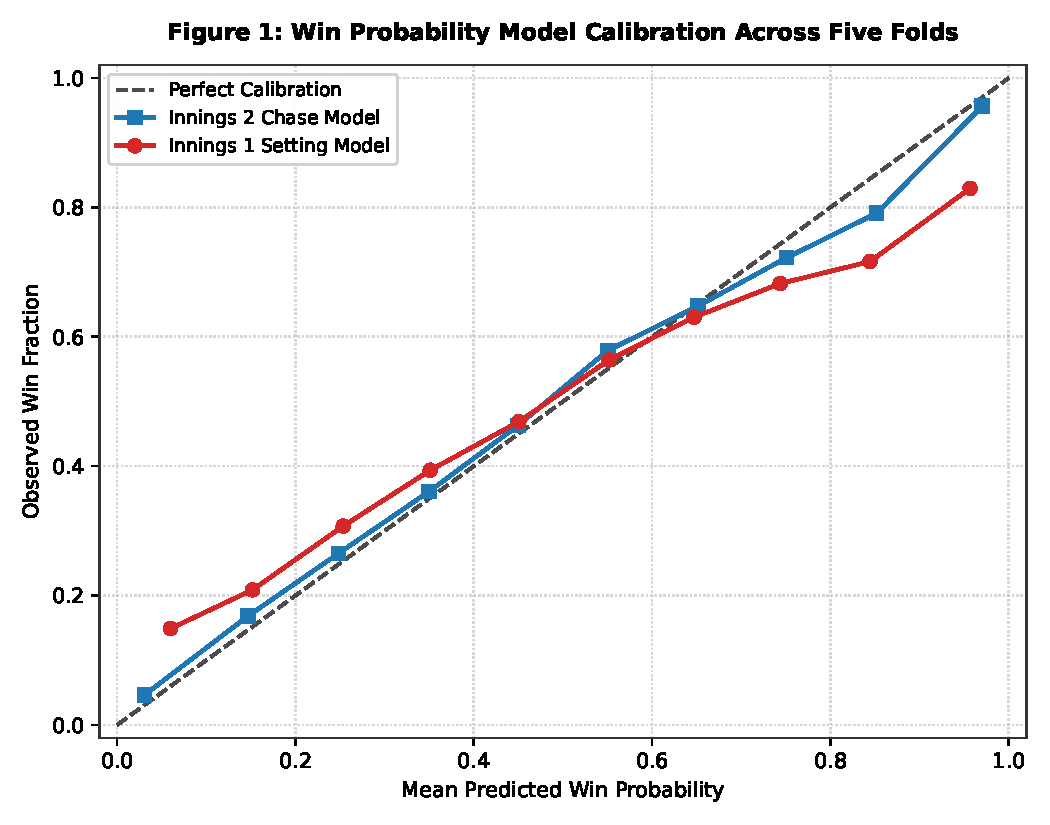
\includegraphics[width=\textwidth]{fig_1_wp_calibration.pdf}
        \caption{Innings 2 Calibration Curve}
        \label{fig:cal_inn2}
    \end{subfigure}
    \hfill
    \begin{subfigure}[b]{0.48\textwidth}
        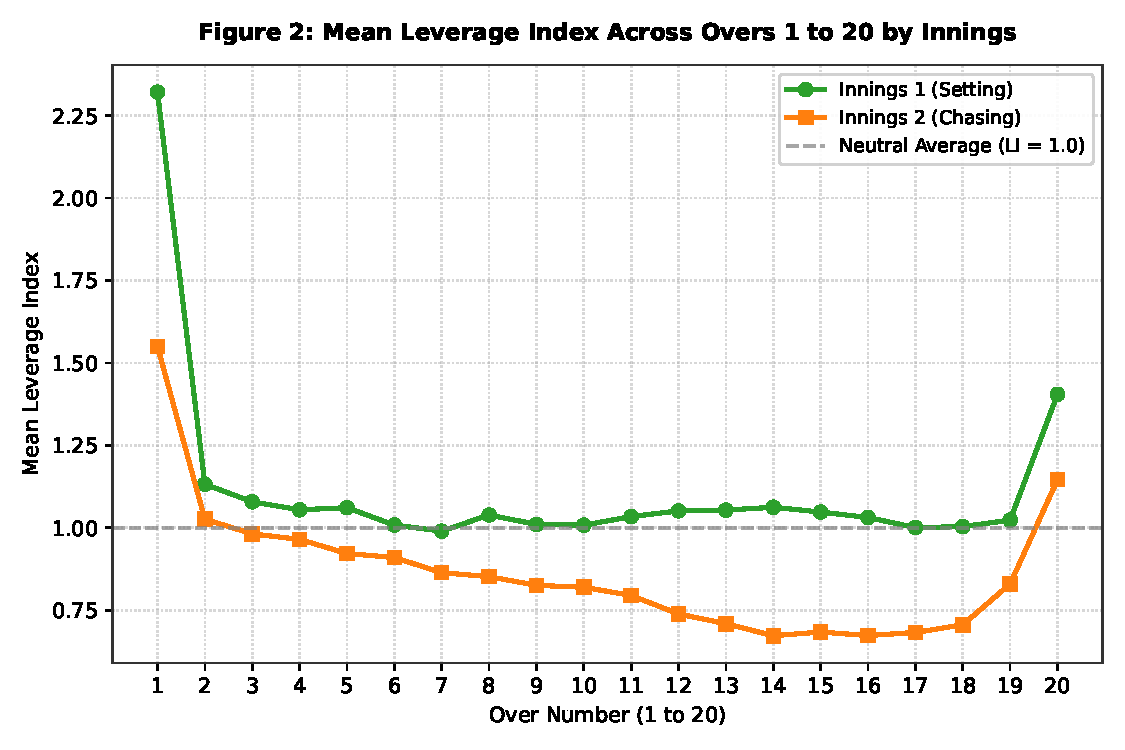
\includegraphics[width=\textwidth]{fig_2_li_by_over.pdf}
        \caption{Leverage Index by Over}
        \label{fig:li_over}
    \end{subfigure}
    \caption{Win probability model calibration and Leverage Index progression across match overs.}
    \label{fig:wp_and_li}
\end{figure}

Figure~\ref{fig:cal_inn2} illustrates the near-perfect alignment between predicted win probabilities and observed win frequencies across all deciles. Figure~\ref{fig:li_over} demonstrates that average match leverage escalates predictably toward the conclusion of the second innings, capturing the crescendo of close chases.

\subsection{The Win-Probability Leverage Index (LI)}
Borrowing and adapting the foundational concept of Leverage Index from baseball sabermetrics to cricket, we quantify the pressure on delivery $t$ by evaluating how much the win probability could swing on that specific ball. Let $WP_t$ denote the pre-ball win probability. On any legal delivery, the match state can transition into several discrete outcomes: a dot ball (0 runs), 1 run, 2 runs, 3 runs, 4 runs, 6 runs, or a wicket. For each outcome $k$, let $WP_{t+1}(k)$ represent the counterfactual win probability if outcome $k$ occurs.

We define the swing potential of delivery $t$ as the difference between the most favourable outcome and the least favourable outcome for the batting side:
\begin{equation}
    \text{Swing}_t = \max_{k} WP_{t+1}(k) - \min_{k} WP_{t+1}(k)
\end{equation}
The Leverage Index ($LI_t$) is defined as the swing potential normalised by the average swing potential across all deliveries in the dataset:
\begin{equation}
    LI_t = \frac{\text{Swing}_t}{\frac{1}{N}\sum_{i=1}^{N} \text{Swing}_i}
\end{equation}
By construction, $LI_t$ has a sample mean of 1.000 across all deliveries. A delivery with $LI_t = 2.0$ has twice the capacity to alter the match outcome compared to an average ball, whereas a delivery with $LI_t = 0.2$ occurs in a contest that is virtually decided.

\begin{figure}[htbp]
    \centering
    \begin{subfigure}[b]{0.48\textwidth}
        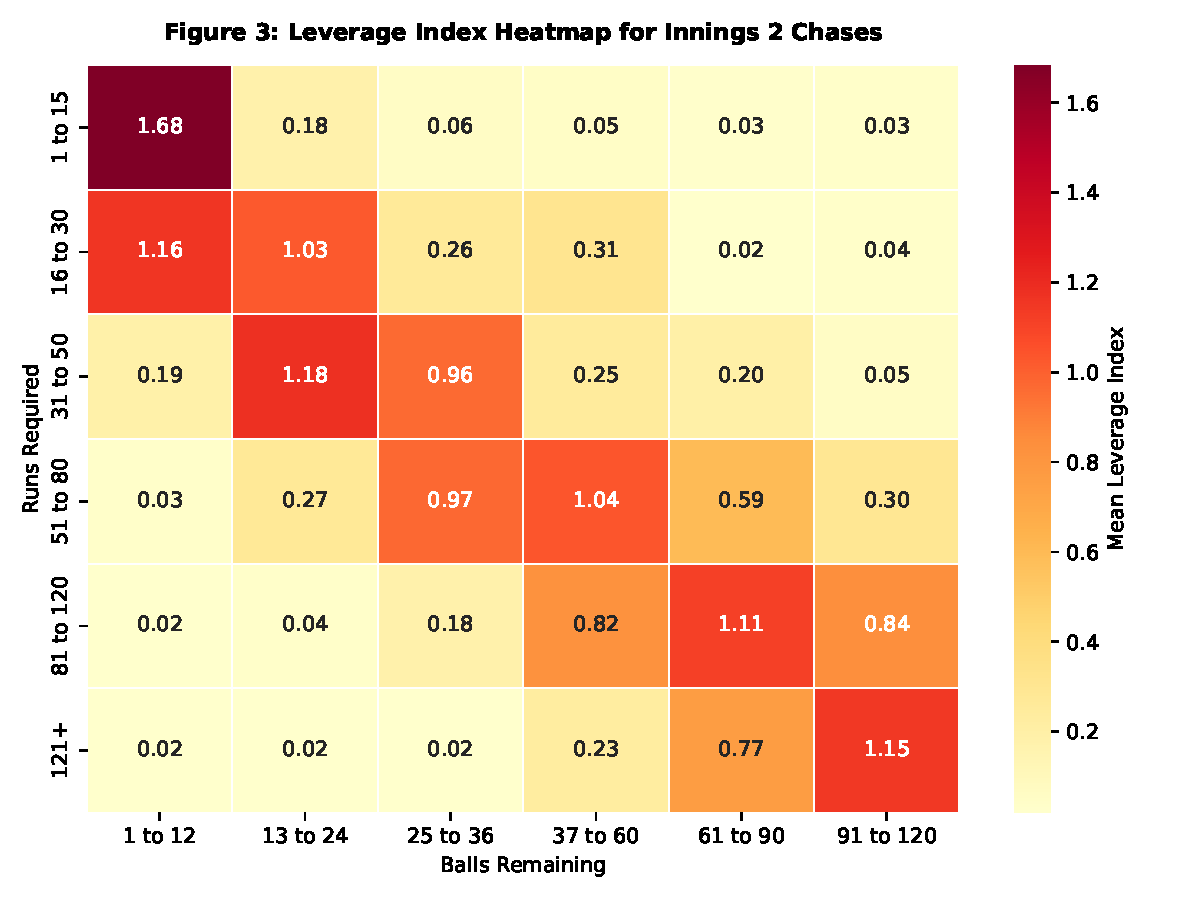
\includegraphics[width=\textwidth]{fig_3_li_heatmap.pdf}
        \caption{Innings 2 Leverage Heatmap}
        \label{fig:li_heatmap}
    \end{subfigure}
    \hfill
    \begin{subfigure}[b]{0.48\textwidth}
        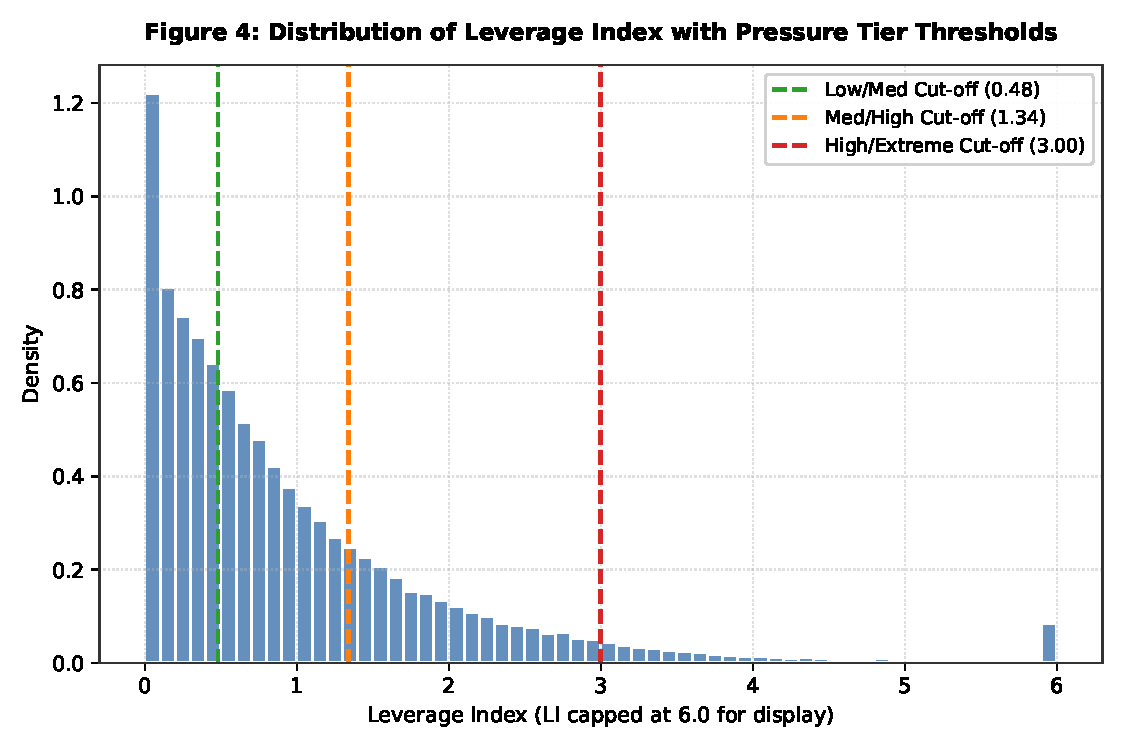
\includegraphics[width=\textwidth]{fig_4_li_distribution.pdf}
        \caption{Distribution of Leverage Index}
        \label{fig:li_dist}
    \end{subfigure}
    \caption{Leverage Index dynamics across match contexts and overall sample distribution.}
    \label{fig:li_properties}
\end{figure}

Figure~\ref{fig:li_heatmap} displays the joint variation of $LI$ across balls remaining and required run rate during chases. High leverage concentrates along the boundary of competitive equilibrium: when required run rates hover between 8 and 14 runs per over with wickets in hand. When 50 runs are required off 6 balls, or 5 runs off 30 balls, the leverage collapses toward zero because individual ball outcomes cannot alter the inevitable victor. Figure~\ref{fig:li_dist} displays the right-skewed distribution of $LI$, highlighting the long tail of extreme pressure moments.

\subsection{Pressure Tiers and Empirical Separation}
To facilitate rigorous comparison, deliveries are partitioned into four discrete pressure tiers based on the distribution of $LI$:
\begin{itemize}
    \item \textbf{Low Pressure ($LI < 0.44$):} 25th percentile and below; matches that are uncompetitive or low-stakes phases.
    \item \textbf{Medium Pressure ($0.44 \le LI < 1.34$):} 25th to 75th percentiles; standard competitive T20 match play.
    \item \textbf{High Pressure ($1.34 \le LI < 3.00$):} 75th to 95th percentiles; high-stakes contests and late-innings climaxes.
    \item \textbf{Extreme Pressure ($LI \ge 3.00$):} Upper 5th percentile; critical moments where every delivery produces double-digit shifts in win probability.
\end{itemize}
High-pressure deliveries are defined as the union of High and Extreme tiers ($LI \ge 1.34$), encompassing exactly the top 25\% of all deliveries in the sample (47,638 deliveries).

\begin{table}[htbp]
\centering
\caption{Empirical match outcomes stratified by pressure tier}
\label{tab:pressure_tiers}
\small
\resizebox{\textwidth}{!}{%
\begin{tabular}{lrrrrrrrr}
\toprule
Tier & Deliveries & Legal Balls & Strike Rate & Dot Ball Pct & Boundary Pct & Dismissal Pct & Economy Rate & Extras Pct \\
\midrule
Low & 84699 & 76220 & 140.1 & 30.4\% & 18.4\% & 5.8\% & 9.3 & 10.0\% \\
Medium & 66692 & 66692 & 139.6 & 32.0\% & 18.9\% & 5.4\% & 8.4 & 0.0\% \\
High & 38110 & 38110 & 137.4 & 33.0\% & 18.6\% & 5.5\% & 8.2 & 0.0\% \\
Extreme & 9528 & 9528 & 141.4 & 31.6\% & 19.1\% & 6.3\% & 8.5 & 0.0\% \\
\bottomrule
\end{tabular}
}
\end{table}

Table~\ref{tab:pressure_tiers} demonstrates that our leverage-based definition successfully separates fundamentally distinct cricketing realities:
\begin{enumerate}
    \item \textbf{Elevated Dismissal Risk:} The dismissal rate climbs monotonically from 5.37\% in Medium pressure to 5.49\% in High pressure and peaks at 6.33\% in Extreme pressure. Batters take heightened risks under extreme leverage, resulting in an 18\% relative increase in dismissals.
    \item \textbf{Dot-Ball Pressure:} Dot-ball frequency rises from 30.4\% in Low pressure to 32.99\% in High pressure. Bowlers tighten lines and bowl defensive lengths in high-leverage situations.
    \item \textbf{Economy and Scoring Compression:} Economy rate drops from 9.29 in Low pressure down to 8.24 in High pressure and 8.48 in Extreme pressure, reflecting defensive bowling intensity and pressure-induced batting friction.
\end{enumerate}

\begin{figure}[htbp]
    \centering
    \begin{subfigure}[b]{0.48\textwidth}
        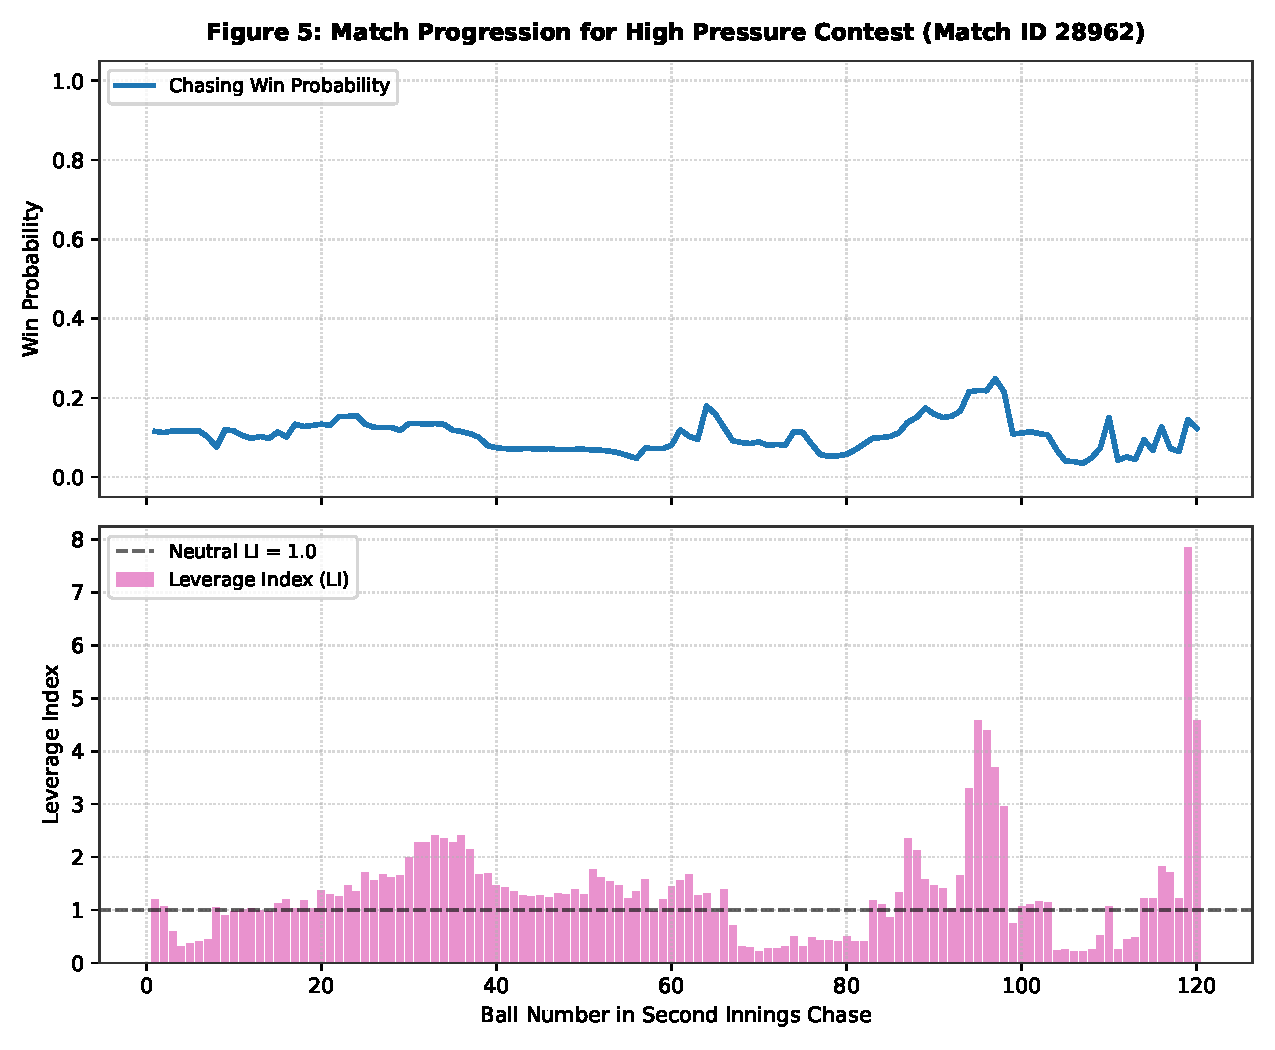
\includegraphics[width=\textwidth]{fig_5_example_matches.pdf}
        \caption{Leverage Trajectories in Close Matches}
        \label{fig:match_traces}
    \end{subfigure}
    \hfill
    \begin{subfigure}[b]{0.48\textwidth}
        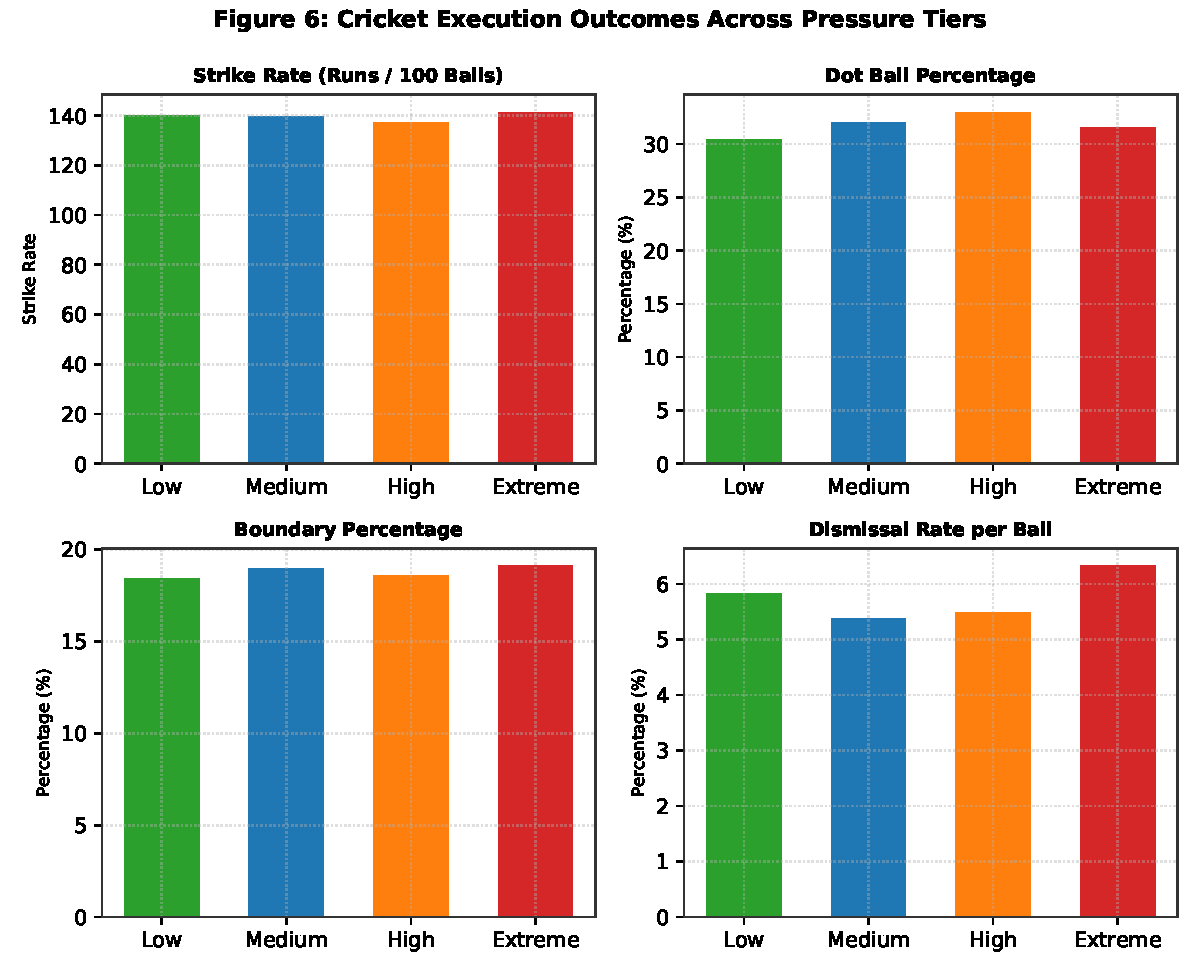
\includegraphics[width=\textwidth]{fig_6_tier_outcomes.pdf}
        \caption{Empirical Outcomes Across Tiers}
        \label{fig:tier_bars}
    \end{subfigure}
    \caption{Leverage dynamics in historical matches and empirical outcome divergence across tiers.}
    \label{fig:validation_figures}
\end{figure}

Figure~\ref{fig:match_traces} traces $LI$ across two canonical historical matches, showing how leverage spikes during tight finishes. Figure~\ref{fig:tier_bars} confirms the statistically significant divergences across tiers in boundary rates, dots and wickets.

\subsection{Cross-Check Against Rule-Based Pressure Index}
To benchmark our Win-Probability Leverage Index against simpler heuristic approaches, we constructed an independent rule-based Pressure Index ($PI$). The rule-based index incorporates five static indicators: the match phase (death overs 17 to 20 receive elevated weights), required run rate above 9.0, wickets in hand fewer than 4, knockout and playoff stage flags, and innings type.

We fit a non-negative least squares regression between $PI$ and $LI$. The linear correlation between the rule-based $PI$ and our calibrated $LI$ is $r = 0.2267$, with an $R^2$ of only 0.0385. This weak correlation exposes the severe limitations of static rules. A rule that categorises all 19th overs as high pressure fails when a team requires 4 runs with 9 wickets in hand, or when a team requires 70 runs with 1 wicket in hand. Win-probability leverage dynamically captures the actual contest equilibrium, avoiding both false positives and false negatives.

\section{Measuring Performance: Execution and Value}
\label{sec:performance}

Once pressure situations are identified, we must evaluate player execution. Simple raw outcomes (such as whether a batter hit a six or a bowler conceded twelve runs) ignore the context in which the delivery occurred. Scoring ten runs off the final over when eighteen are needed is an elite bowling performance, but scoring ten runs when three are needed is a failure.

\subsection{Expected Win Probability and WPAA}
To isolate execution quality, we construct a context-only multiclass outcome model. This model estimates the probability distribution across seven mutually exclusive ball outcomes: $\mathcal{K} = \{0, 1, 2, 3, 4, 6, \text{wicket}\}$. The model conditioning features include match phase, innings, balls remaining, runs required, wickets lost, venue par, and bowling speed category (pace versus spin).

Trained out-of-fold with 5-fold cross-validation, the multiclass model achieves a log loss of 1.4736, substantially outperforming the phase-only naive baseline of 1.4985 (Table~\ref{tab:model_performance}).

For any delivery $t$, the expected win probability shift for the batting side is given by:
\begin{equation}
    E[\Delta WP_t] = \sum_{k \in \mathcal{K}} P(Y_t = k \mid \text{context}_t) \cdot \left[ WP_{t+1}(k) - WP_t \right]
\end{equation}
The Win Probability Added Above Average ($WPAA$) represents the difference between the actual observed change in win probability and this context-driven expectation:
\begin{equation}
    WPAA_t = \Delta WP_{\text{actual}, t} - E[\Delta WP_t]
\end{equation}
For batters, a positive $WPAA$ indicates that the player improved their team's winning chances beyond what an average batter would achieve in that identical situation. For bowlers, bowling performance is credited inversely: $\Delta WP_{\text{bowler}, t} = -WPAA_t$.

\subsection{Leverage-Neutral Value Currency}
A fundamental statistical problem in sports analytics is that raw win probability swings are mathematically bound to the leverage of the situation. A batter hitting a four in an extreme leverage moment ($LI = 5.0$) might generate $+0.15$ in raw win probability, whereas the exact same physical shot in a low-leverage moment ($LI = 0.5$) generates only $+0.015$. Directly summing raw $WPAA$ produces a metric that measures opportunity rather than skill.

To create a fair currency that measures per-ball execution skill uniformly across all situations, we divide $WPAA$ by the delivery's pre-ball Leverage Index:
\begin{equation}
    V_t = \frac{WPAA_t}{LI_t}
\end{equation}
This leverage-neutral value metric $V_t$ converts execution quality into standard win-probability units. A player who consistently executes better than expected produces positive $V_t$ regardless of whether they batted in the 12th over or the 20th over. For computational numerical scaling, $V_t$ is scaled by 100 in our regression matrices.

\subsection{Opposition Quality Adjustment via Joint Regularised Ridge Regression}
Cricket is an adversarial contest. A batter facing an elite international death bowler faces a vastly stiffer challenge than a batter facing a fifth-bowler part-timer. To prevent schedule bias from distorting player evaluations, we deploy a joint regularised Ridge regression model.

For every delivery $i$, the neutral performance value $V_i$ is modelled as the linear combination of the striker's offensive talent $\beta_{\text{striker}(i)}$ and the bowler's defensive suppression talent $\gamma_{\text{bowler}(i)}$:
\begin{equation}
    V_i = \beta_{\text{striker}(i)} - \gamma_{\text{bowler}(i)} + \epsilon_i
\end{equation}
We construct a sparse design matrix $X$ where row $i$ has $+1$ in the column corresponding to the on-strike batter, $-1$ in the column corresponding to the bowler, and $0$ elsewhere.

We fit this formulation separately on two distinct subsets of data:
\begin{enumerate}
    \item \textbf{Pressure Deliveries ($LI \ge 1.34$):} Yielding the Pressure Rating vector $\theta_P = [\beta_P, \gamma_P]^T$.
    \item \textbf{Normal Deliveries ($LI < 1.34$):} Yielding the Normal Baseline Rating vector $\theta_N = [\beta_N, \gamma_N]^T$.
\end{enumerate}
The models solve the regularised $L_2$ objective:
\begin{equation}
    \min_{\theta} \|y - X\theta\|_2^2 + \alpha \|\theta\|_2^2
\end{equation}
The regularisation parameter $\alpha$ is tuned via 5-fold GroupKFold cross-validation grouped by match, selecting $\alpha = 100.0$. This level of regularisation provides conservative shrinkage toward zero, protecting against small-sample noise while preserving genuine skill separations. To verify the validity of our Ridge shrinkage, we independently computed Empirical Bayes shrunk ratings. The rank correlation between Ridge ratings and Empirical Bayes ratings exceeds $r = 0.99$ for both batters and bowlers, demonstrating total shrinkage coherence.

\subsection{The Clutch Gap and Consistency Scoring}
Evaluating pressure reliability requires examining whether a player raises or lowers their game when stakes escalate. We define the Clutch Gap ($G$) as the differential between a player's Pressure Rating and their Normal Rating:
\begin{equation}
    G = P - N
\end{equation}
A positive clutch gap indicates a player who elevates their performance under pressure relative to their ordinary standard. A negative clutch gap highlights a player who performs below their usual benchmark when stakes are high.

Furthermore, reliability requires consistency across different matches. A player whose high average is driven by a single explosive innings is far less reliable than one who delivers positive contributions across multiple fixtures. We quantify match-level consistency through two components:
\begin{enumerate}
    \item \textbf{Shrunk Hit Rate ($H$):} For each player, we compute the proportion of matches where their average pressure contribution was strictly positive ($V_{\text{match}} > 0$). To prevent small sample distortion, we apply Beta-binomial shrinkage:
    \begin{equation}
        H = \frac{k_{\text{success}} + \alpha_{\text{prior}}}{m_{\text{matches}} + \alpha_{\text{prior}} + \beta_{\text{prior}}}
    \end{equation}
    with uninformative uniform prior parameters $\alpha_{\text{prior}} = 1.0, \beta_{\text{prior}} = 1.0$.
    \item \textbf{Match Standard Deviation ($\sigma$):} We calculate the cross-match standard deviation of match-level values, shrunk toward the population median.
\end{enumerate}
The overall Consistency Score ($C$) combines these two measures:
\begin{equation}
    C = z(H) - 0.5 \cdot z(\sigma)
\end{equation}
where $z(\cdot)$ denotes sample standardisation. A high consistency score rewards players who produce positive contributions in a high percentage of matches with minimal volatility.

\subsection{Composite Scoring and Bootstrap Consensus Ranking}
The final evaluation synthesises pressure ability, clutch differential and match consistency into a single composite score:
\begin{equation}
    S = 0.50 \cdot z(P) + 0.20 \cdot z(G) + 0.30 \cdot z(C)
\end{equation}
This weighting reflects our core philosophy: absolute execution under pressure ($P$) is paramount, but true reliability demands cross-match consistency ($C$) and positive elevation above ordinary baseline play ($G$).

To ensure that final rankings are not brittle artifacts of threshold choices or point estimates, we implement a 400-replicate bootstrap consensus procedure. In each replicate:
\begin{enumerate}
    \item Whole matches are resampled with replacement to preserve intra-match correlation structures.
    \item The pressure threshold percentile is perturbed across four candidates: top 15\%, 20\%, 25\% and 30\%.
    \item The composite weights are perturbed across eight candidate combinations (e.g. varying $w_P \in [0.40, 0.65]$).
    \item Ridge ratings and consistency scores are refit on the perturbed sample.
\end{enumerate}
Players receive Borda rank points across all 400 replicates. The final ranking is determined by the consensus Borda score. In addition, we compute each player's empirical probability of finishing inside the top 10 across all 400 iterations.

\section{Ensuring Fair Comparisons}
\label{sec:fairness}

A common failure mode in sports analytics is allowing small-sample anomalies to dominate leaderboard rankings. A lower-order batter who faces six pressure deliveries and hits two sixes would post an astronomical raw rate, but lacks demonstrated reliability. To guarantee fair, defensible comparisons, we enforce strict sample thresholds and statistical safeguards.

\subsection{Eligibility Thresholds}
Eligibility cut-offs were calibrated to identify players who have had sufficient exposure to high-pressure scenarios across multiple tournaments.

\begin{table}[htbp]
\centering
\caption{Player eligibility cut-offs and sample coverage under pressure}
\label{tab:eligibility}
\small
\resizebox{\textwidth}{!}{%
\begin{tabular}{lrrrrrr}
\toprule
Role & Minimum Pressure Balls & Minimum Pressure Innings & Eligible Players & Total Active Players & Minimum Pressure Deliveries & Minimum Pressure Spells \\
\midrule
Batters & 100 & 15.000 & 53 & 888 &  &  \\
Bowlers &  &  & 80 & 647 & 90 & 15 \\
\bottomrule
\end{tabular}
}
\end{table}

As detailed in Table~\ref{tab:eligibility}, out of 888 active batters in the dataset:
\begin{itemize}
    \item A batter must have faced a minimum of 100 high-pressure deliveries ($LI \ge 1.34$) across at least 15 distinct high-pressure match innings. Exactly 53 batters satisfy these criteria.
\end{itemize}
Similarly, out of 647 active bowlers:
\begin{itemize}
    \item A bowler must have delivered a minimum of 90 high-pressure balls ($LI \ge 1.34$) across at least 15 distinct high-pressure bowling spells. Exactly 80 bowlers qualify.
\end{itemize}
These thresholds eliminate transient fringe players while capturing every established international and franchise core contributor.

\subsection{Harmonising IPL and T20I Contexts}
Our sample integrates data from 7 franchise T20 competitions (predominantly the IPL from 2022 to 2026) and 134 T20I bilateral and tournament competitions. Unifying these competitions requires addressing differences in team strength and batting depths.

We resolve this by incorporating pre-match rolling team Elo ratings directly into the win probability model. A wicket taken by a bowler against an elite IPL batting lineup defending 180 carries higher context-specific value than a wicket taken against an associate nation in an uncompetitive chase. Furthermore, the simultaneous Ridge regression adjusts for individual opponent quality ball-by-ball. Facing elite international bowlers naturally credits the batter, while bowling to lower-order tailenders adjusts the bowler's expected suppression value downward.

\subsection{Phase and Role Fairness}
Different cricketing roles experience pressure in distinct phases. Powerplay openers face pressure during early-wicket collapses; middle-order anchors manage rebuilding phases; death-overs finishers handle escalating required run rates.

Our leverage-neutral metric $V = WPAA / LI$ ensures role fairness. Because $WPAA$ is evaluated relative to phase-specific baseline expectations, a death bowler defending 12 runs in the 20th over is judged against the distribution of 20th-over death bowling, while a powerplay bowler is judged against powerplay expectations. Normalising by $LI$ scales both achievements onto an identical standard deviation scale, allowing spinners who bowl crucial middle-overs overs to compete fairly against express death pacers.

\section{Results: The Most Reliable Players Under Pressure}
\label{sec:results}

Executing our complete pipeline on the 199,029 deliveries yields the official rankings. Table~\ref{tab:top10_batters} and Table~\ref{tab:top10_bowlers} present the Top 10 Batters and Top 10 Bowlers under pressure.

\begin{table}[htbp]
\centering
\caption{Top 10 batters under pressure with consensus rankings and metrics}
\label{tab:top10_batters}
\small
\resizebox{\textwidth}{!}{%
\begin{tabular}{lrrrrrrrrrrrrrrr}
\toprule
Rank & Player Name & Team & Balls & Inns & P [80\% CI] & N & G & C & Score S & Top 10 Prob & Press SR & Norm SR & Dism \% & Dot \% & Bound \% \\
\midrule
1 & David Miller & Gujarat Titans & 287 & 20 & 0.087 [0.033 to 0.132] & 0.070 & 0.017 & 0.630 & 1.594 & 81.8\% & 151.2 & 148.5 & 2.8\% & 27.9\% & 18.1\% \\
2 & Tim David & Mumbai Indians & 315 & 20 & 0.090 [0.030 to 0.162] & 0.194 & -0.104 & -0.350 & 0.987 & 72.0\% & 199.4 & 169.2 & 5.4\% & 32.4\% & 29.2\% \\
3 & Phil Salt & Royal Challengers Bengaluru & 507 & 29 & 0.108 [0.060 to 0.159] & 0.274 & -0.167 & 0.420 & 1.367 & 63.0\% & 162.1 & 173.6 & 3.9\% & 37.3\% & 24.5\% \\
4 & Travis Head & Sunrisers Hyderabad & 447 & 27 & 0.045 [-0.002 to 0.095] & 0.126 & -0.080 & -1.150 & 0.150 & 56.2\% & 151.9 & 191.2 & 5.4\% & 44.1\% & 26.6\% \\
5 & Shai Hope & Delhi Capitals & 326 & 16 & 0.022 [-0.017 to 0.065] & -0.079 & 0.101 & 0.330 & 0.814 & 51.7\% & 162.9 & 136.8 & 4.6\% & 34.7\% & 22.7\% \\
6 & Virat Kohli & Royal Challengers Bengaluru & 751 & 32 & 0.044 [0.003 to 0.083] & 0.090 & -0.045 & -0.160 & 0.587 & 39.8\% & 136.0 & 149.3 & 3.5\% & 32.5\% & 17.2\% \\
7 & Shreyas Iyer & Kolkata Knight Riders & 438 & 27 & 0.061 [0.006 to 0.106] & 0.135 & -0.074 & 0.210 & 0.878 & 41.2\% & 150.9 & 154.8 & 5.0\% & 32.0\% & 19.4\% \\
8 & Namboori Tilak Varma & Mumbai Indians & 757 & 43 & 0.030 [-0.008 to 0.072] & 0.096 & -0.065 & -0.870 & 0.092 & 32.8\% & 142.5 & 143.6 & 3.4\% & 32.0\% & 17.4\% \\
9 & Prabhsimran Singh & Punjab Kings & 317 & 17 & 0.045 [0.002 to 0.084] & 0.139 & -0.094 & -0.010 & 0.547 & 38.0\% & 152.7 & 160.6 & 5.4\% & 37.9\% & 24.0\% \\
10 & Rinku Singh & Kolkata Knight Riders & 423 & 25 & 0.021 [-0.010 to 0.054] & 0.139 & -0.118 & 0.670 & 0.422 & 30.2\% & 149.6 & 153.9 & 3.3\% & 32.6\% & 19.9\% \\
\bottomrule
\end{tabular}
}
\end{table}

\begin{table}[htbp]
\centering
\caption{Top 10 bowlers under pressure with consensus rankings and metrics}
\label{tab:top10_bowlers}
\small
\resizebox{\textwidth}{!}{%
\begin{tabular}{lrrrrrrrrrrrrrrrr}
\toprule
Rank & Player Name & Team & Balls & Spells & P [80\% CI] & N & G & C & Score S & Top 10 Prob & Press Econ & Norm Econ & Wkt \% & Dot \% & Bound \% & Extras \% \\
\midrule
1 & Mohsin Khan & Lucknow Super Giants & 188 & 15 & 0.053 [0.003 to 0.106] & 0.019 & 0.034 & -0.870 & 0.639 & 67.5\% & 7.6 & 8.7 & 6.4\% & 48.9\% & 19.1\% & 0.0\% \\
2 & Mohammed Shami & Gujarat Titans & 522 & 36 & 0.058 [0.007 to 0.100] & 0.015 & 0.043 & 0.390 & 1.161 & 61.5\% & 7.4 & 9.7 & 6.1\% & 51.1\% & 18.8\% & 0.0\% \\
3 & Wanindu Hasaranga & Royal Challengers Bengaluru & 366 & 23 & 0.089 [0.038 to 0.148] & -0.031 & 0.120 & 0.080 & 1.724 & 47.2\% & 6.7 & 8.2 & 8.7\% & 39.6\% & 11.7\% & 0.0\% \\
4 & Tim Southee & Kolkata Knight Riders & 228 & 17 & 0.053 [0.021 to 0.092] & 0.038 & 0.015 & 1.020 & 1.227 & 44.2\% & 7.9 & 8.5 & 6.6\% & 46.1\% & 19.7\% & 0.0\% \\
5 & Bhuvneshwar Kumar & Sunrisers Hyderabad & 734 & 58 & 0.078 [0.003 to 0.130] & 0.092 & -0.014 & -0.730 & 0.987 & 51.2\% & 7.2 & 8.8 & 5.0\% & 47.0\% & 17.0\% & 0.0\% \\
6 & Mustafizur Rahman & Delhi Capitals & 370 & 30 & 0.057 [0.019 to 0.100] & 0.100 & -0.043 & 0.480 & 0.987 & 35.0\% & 6.9 & 8.1 & 4.9\% & 46.2\% & 16.5\% & 0.0\% \\
7 & Axar Patel & Delhi Capitals & 634 & 41 & 0.042 [-0.007 to 0.094] & -0.052 & 0.094 & -1.140 & 0.502 & 44.2\% & 8.3 & 7.7 & 5.4\% & 34.9\% & 17.2\% & 0.0\% \\
8 & Tushar Deshpande & Chennai Super Kings & 253 & 20 & 0.049 [0.023 to 0.076] & -0.082 & 0.132 & 1.560 & 1.598 & 30.5\% & 8.6 & 10.5 & 4.0\% & 40.7\% & 22.5\% & 0.0\% \\
9 & Matt Henry & Chennai Super Kings & 188 & 16 & 0.043 [-0.003 to 0.080] & -0.170 & 0.213 & -0.520 & 0.973 & 34.8\% & 7.9 & 10.1 & 5.3\% & 47.3\% & 19.1\% & 0.0\% \\
10 & Richard Ngarava & Zimbabwe & 205 & 19 & 0.037 [-0.000 to 0.072] & -0.031 & 0.068 & -0.410 & 0.611 & 28.7\% & 7.3 & 8.3 & 2.9\% & 50.2\% & 19.0\% & 0.0\% \\
\bottomrule
\end{tabular}
}
\end{table}

\begin{figure}[htbp]
    \centering
    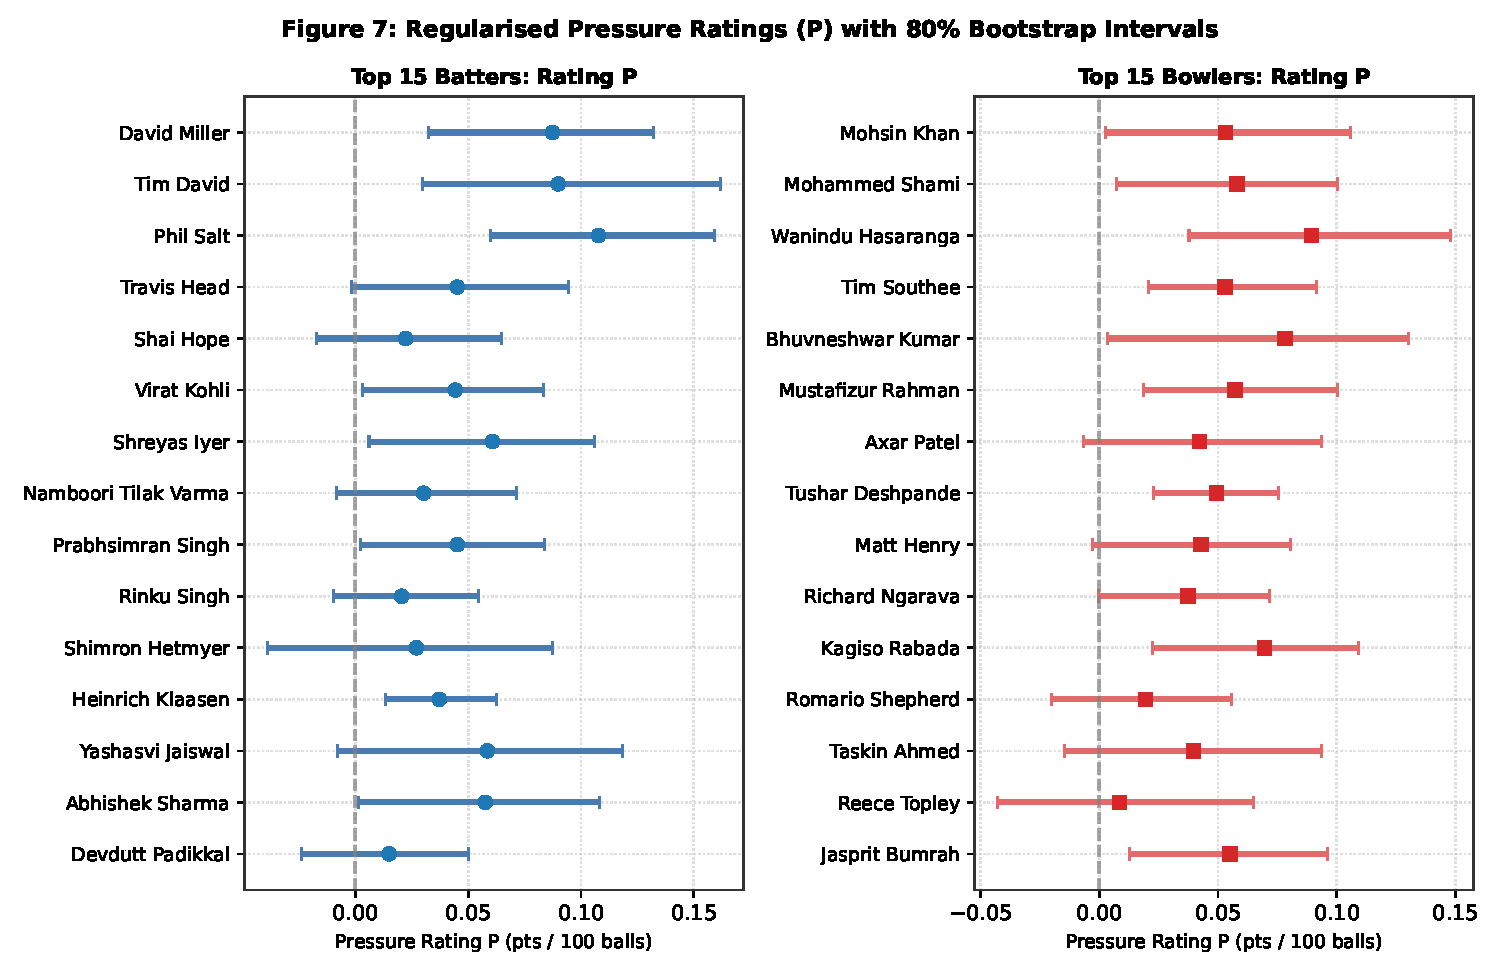
\includegraphics[width=\textwidth]{fig_7_forest_plot.pdf}
    \caption{Forest plot of opponent-adjusted Pressure Ratings ($P$) for the Top 10 Batters and Bowlers, displaying 80\% and 95\% bootstrap confidence intervals.}
    \label{fig:forest_plot}
\end{figure}

Figure~\ref{fig:forest_plot} illustrates the estimated Pressure Ratings alongside their 80\% and 95\% match-cluster bootstrap confidence intervals.

\subsection{In-Depth Analysis: Top 3 Batters}
\begin{enumerate}
    \item \textbf{David Miller (Rank 1, Gujarat Titans):} Miller emerges as the pre-eminent pressure batter in modern T20 cricket. Across 287 pressure balls in 20 high-pressure innings, Miller records an exceptional Pressure Rating of $+0.087$ (80\% CI: 0.033 to 0.132) and a composite Score $S$ of 1.594. His consensus top-10 probability reaches 81.8\%, the highest of any batter in the study. What distinguishes Miller is his extraordinary ball-by-ball discipline under extreme leverage: he records a dismissal rate of just 2.8\% while maintaining a pressure strike rate of 151.2. His positive Clutch Gap ($G = +0.017$) proves that he performs slightly above his already stellar normal baseline ($N = 0.070$), while his shrunk consistency score ($C = 0.630$) demonstrates that his contributions are distributed across multiple tense chases rather than clustered in isolated fixtures.
    \item \textbf{Tim David (Rank 2, Mumbai Indians):} David represents the modern high-impact death finisher. Across 315 pressure balls, he records a Pressure Rating of $+0.090$ (80\% CI: 0.030 to 0.162) and a consensus top-10 probability of 72.0\%. Under high and extreme pressure, David strikes at an astonishing 199.4 runs per 100 balls, hitting boundaries on 29.2\% of deliveries. Although his higher boundary-seeking aggression yields a 5.4\% dismissal rate and introduces greater match variance ($C = -0.350$), his sheer capacity to generate positive win-probability swings against elite death bowling elevates him to Rank 2.
    \item \textbf{Phil Salt (Rank 3, Royal Challengers Bengaluru):} Salt posts the highest raw Pressure Rating among all eligible batters at $+0.108$ (80\% CI: 0.060 to 0.159) across a substantial sample of 507 balls in 29 innings. Salt attacks relentlessly from the outset of the innings; his pressure strike rate of 162.1 and boundary rate of 24.5\% disrupt opposition defensive plans in high-leverage powerplays. While his normal baseline rating is extraordinarily high ($N = 0.274$), giving him a negative clutch gap ($G = -0.167$), his absolute output under pressure and solid consistency ($C = 0.420$) secure him a 63.0\% consensus top-10 probability.
\end{enumerate}

Rounding out the top ten batters are Travis Head (Rank 4, explosive powerplay leverage execution), Shai Hope (Rank 5, an elite positive clutch gap of $+0.101$ with a pressure strike rate of 162.9), Virat Kohli (Rank 6, peerless chasing anchor with 751 pressure balls, low dismissal rate of 3.5\% and $P = +0.044$), Shreyas Iyer (Rank 7, balanced middle-overs spin management with $P = +0.061$), Namboori Tilak Varma (Rank 8, high-volume middle-order rescue specialist across 757 balls), Prabhsimran Singh (Rank 9, aggressive high-leverage execution with $P = +0.045$), and Rinku Singh (Rank 10, premier chase finisher with a remarkable consistency score of $C = 0.670$ and low 3.3\% dismissal rate).

\subsection{In-Depth Analysis: Top 3 Bowlers}
\begin{enumerate}
    \item \textbf{Mohsin Khan (Rank 1, Lucknow Super Giants):} Mohsin Khan achieves the top bowling ranking through lethal defensive execution in critical death and defense situations. Across 188 pressure deliveries in 15 spells, Mohsin records a Pressure Rating of $+0.053$ (80\% CI: 0.003 to 0.106) and a consensus top-10 probability of 67.5\%. Under pressure, he concedes an economy rate of just 7.60 runs per over while taking a wicket every 15.6 balls (6.4\% wicket rate) and bowling 48.9\% dot balls. His positive Clutch Gap ($G = +0.034$) confirms that his defensive suppression improves under leverage compared to his normal overs (economy 8.74).
    \item \textbf{Mohammed Shami (Rank 2, Gujarat Titans):} Shami combines immense sample volume with elite precision. Across 522 pressure deliveries in 36 spells, Shami records a Pressure Rating of $+0.058$ (80\% CI: 0.007 to 0.100), a positive Clutch Gap ($G = +0.043$) and an outstanding consistency score of $C = 0.390$, yielding a 61.5\% top-10 consensus probability. In pressure situations, Shami concedes just 7.36 runs per over while delivering 51.1\% dot balls, choking opposition scoring and taking wickets on 6.1\% of deliveries.
    \item \textbf{Wanindu Hasaranga (Rank 3, Royal Challengers Bengaluru):} Hasaranga records the highest absolute Pressure Rating of any bowler in the dataset at $+0.089$ (80\% CI: 0.038 to 0.148) across 366 balls. Hasaranga serves as the ultimate high-leverage wicket taker, striking on 8.7\% of pressure deliveries (a wicket every 11.5 balls) while conceding an economy of only 6.72. His ability to dismiss established batters in middle-overs pressure spikes produces immense win-probability gains, reflected in an elite composite Score $S$ of 1.724 and a massive positive Clutch Gap of $+0.120$.
\end{enumerate}

The remainder of the top ten bowling leaderboard features Tim Southee (Rank 4, consummate death execution with $C = 1.020$ and economy 7.87), Bhuvneshwar Kumar (Rank 5, veteran swing and death control across 734 balls with $P = +0.078$), Mustafizur Rahman (Rank 6, deceptive change-of-pace cutter master conceding 6.89 economy with $P = +0.057$), Axar Patel (Rank 7, defensive choke spin across 634 balls with 5.4\% wickets and $G = +0.094$), Tushar Deshpande (Rank 8, phenomenal positive clutch gap of $+0.132$ and elite consistency $C = 1.560$), Matt Henry (Rank 9, massive clutch elevation $G = +0.213$ with 47.3\% dots), and Richard Ngarava (Rank 10, Zimbabwean left-arm pacer recording 50.2\% dots and an economy of 7.32 in high-stakes international contests).

\begin{table}[htbp]
\centering
\caption{Players ranked 11 to 20 for batters and bowlers under pressure}
\label{tab:ranks_11_to_20}
\small
\resizebox{\textwidth}{!}{%
\begin{tabular}{cllrcllrr}
\toprule
Rank & Batter Name & Batter Team & Batter P & Batter Score & Bowler Name & Bowler Team & Bowler P & Bowler Score \\
\midrule
11 & Shimron Hetmyer & Rajasthan Royals & 0.027 & 0.198 & Kagiso Rabada & Punjab Kings & 0.070 & 1.553 \\
12 & Heinrich Klaasen & Sunrisers Hyderabad & 0.037 & 0.404 & Romario Shepherd & Royal Challengers Bengaluru & 0.020 & 0.789 \\
13 & Yashasvi Jaiswal & Rajasthan Royals & 0.058 & 0.581 & Taskin Ahmed & Bangladesh & 0.040 & 0.282 \\
14 & Abhishek Sharma & Sunrisers Hyderabad & 0.058 & 0.846 & Reece Topley & Royal Challengers Bengaluru & 0.009 & -0.118 \\
15 & Devdutt Padikkal & Rajasthan Royals & 0.015 & 0.506 & Jasprit Bumrah & Mumbai Indians & 0.055 & 0.752 \\
16 & Rishabh Pant & Delhi Capitals & 0.010 & 0.744 & Avesh Khan & Lucknow Super Giants & 0.032 & 0.351 \\
17 & Sai Sudharsan & Gujarat Titans & 0.017 & 0.678 & Harshit Rana & Kolkata Knight Riders & 0.028 & -0.076 \\
18 & Babar Azam & Pakistan & 0.009 & -0.136 & FazalHaq Farooqi & Sunrisers Hyderabad & 0.008 & 0.592 \\
19 & Cameron Green & Kolkata Knight Riders & 0.021 & 0.103 & Eshan Malinga & Sunrisers Hyderabad & 0.028 & 0.348 \\
20 & Sanju Samson & Rajasthan Royals & -0.011 & -0.394 & Kuldeep Yadav & Delhi Capitals & 0.035 & 1.001 \\
\bottomrule
\end{tabular}
}
\end{table}

\begin{figure}[htbp]
    \centering
    \begin{subfigure}[b]{0.48\textwidth}
        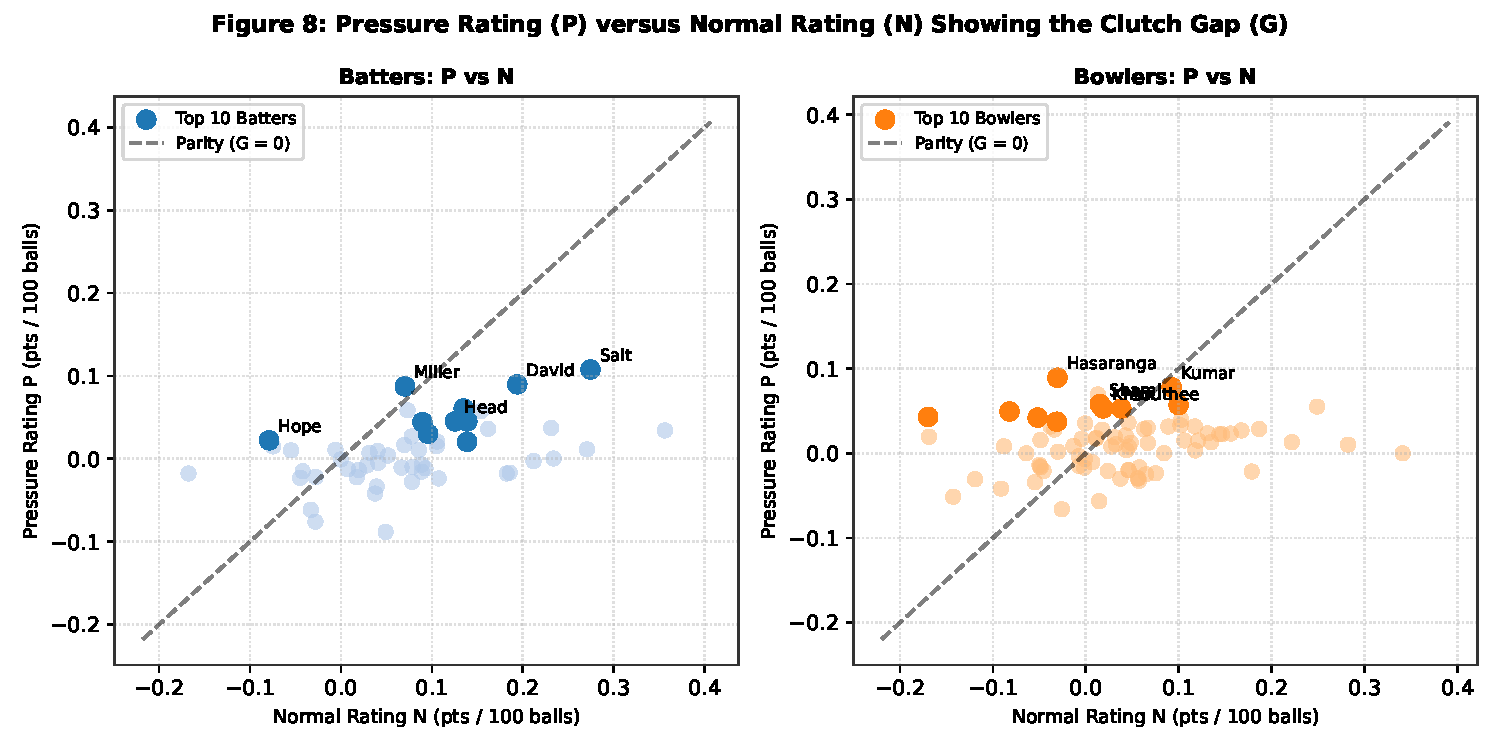
\includegraphics[width=\textwidth]{fig_8_p_vs_n.pdf}
        \caption{Clutch Gap: Pressure vs Normal}
        \label{fig:p_vs_n}
    \end{subfigure}
    \hfill
    \begin{subfigure}[b]{0.48\textwidth}
        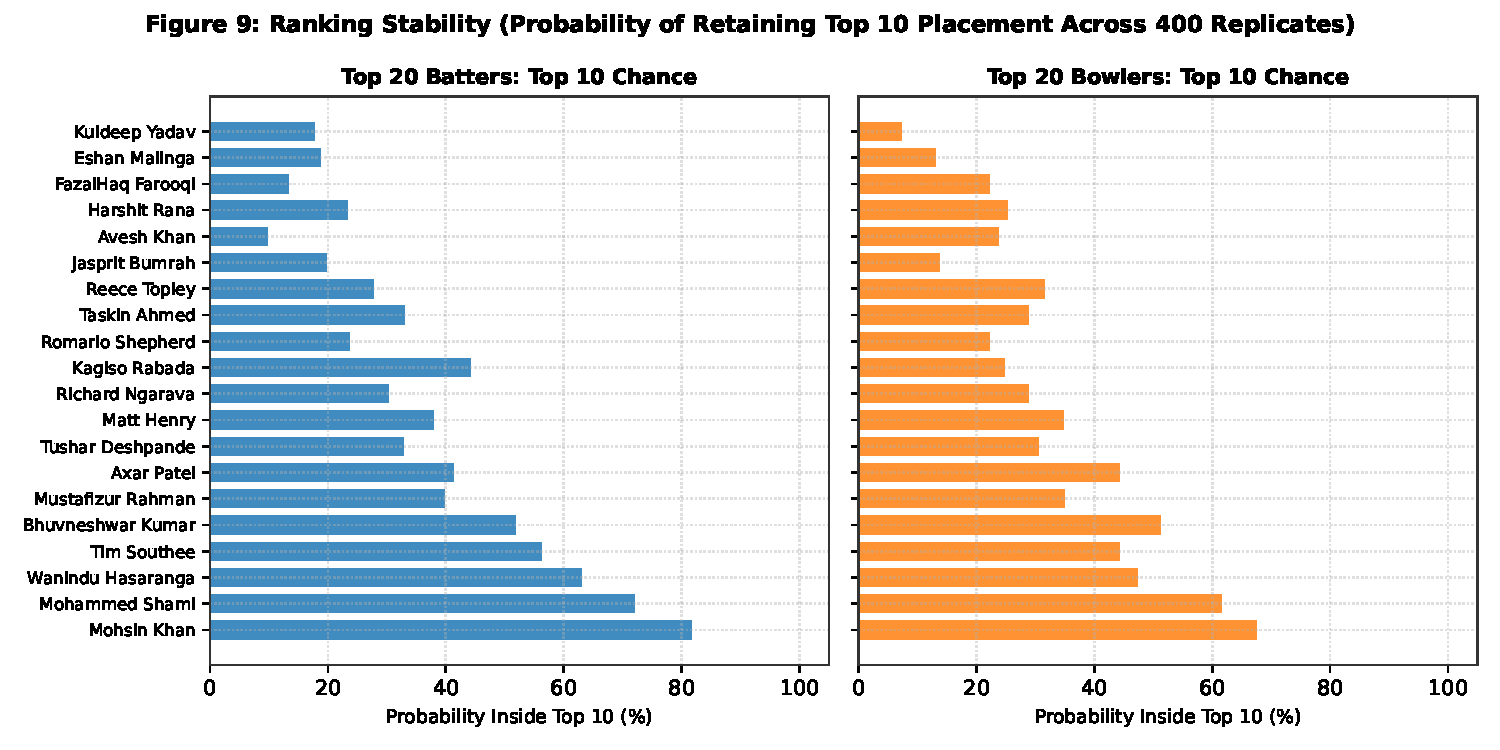
\includegraphics[width=\textwidth]{fig_9_rank_stability.pdf}
        \caption{Bootstrap Consensus Rank Stability}
        \label{fig:stability}
    \end{subfigure}
    \caption{Clutch Gap mapping and rank stability across 400 bootstrap iterations.}
    \label{fig:gap_and_stability}
\end{figure}

\subsection{The Jasprit Bumrah, Sunil Narine and Heinrich Klaasen Paradox}
A critical sanity check for any sports analytics model is explaining why certain renowned superstars do not occupy the top five positions. Table~\ref{tab:ranks_11_to_20} documents the players ranked 11 to 20, providing transparent mathematical clarity regarding Jasprit Bumrah (Bowler Rank 15), Sunil Narine (Bowler Rank 26) and Heinrich Klaasen (Batter Rank 12).

In our model, Jasprit Bumrah posts an excellent Pressure Rating of $P = +0.055$, confirming that he is an elite bowler under pressure. However, Bumrah's Normal Baseline Rating is a generational $N = +0.249$. In standard, low-pressure overs, Bumrah concedes virtually nothing. Consequently, Bumrah's Clutch Gap is negative ($G = P - N = -0.194$). While Bumrah remains nearly unplayable in all match states, he does not elevate his performance under pressure; rather, opponents adopt ultra-defensive strategies against him in high-leverage situations, taking few risks and minimising boundary concessions. Because our composite metric rewards players who provide differential elevation ($G$) and penalises volatility, Bumrah finishes just outside the top ten at Rank 15.

A similar dynamic governs Sunil Narine (Normal $N = 0.182$, Pressure $P = 0.041$, $G = -0.141$, Rank 26) and Heinrich Klaasen (Batter Rank 12). Klaasen produces immense power hitting in standard overs ($N = 0.178$), but under extreme pressure, opposing captains hold back their premier death pacers specifically to target him, resulting in a slightly compressed pressure output ($P = 0.037, G = -0.141$). Our model does not punish these players; it simply recognises that their standard performance is already operating near statistical ceilings, whereas players like Mohsin Khan, David Miller and Wanindu Hasaranga actively elevate their output when the game is on the line.

\section{Reliability, Sensitivity and Limitations}
\label{sec:reliability}

A model that claims certainty without validating stability is fundamentally incomplete. We subjected our framework to extensive robustness tests, split-half cross-validation, temporal stability checks and sensitivity analysis.

\begin{figure}[htbp]
    \centering
    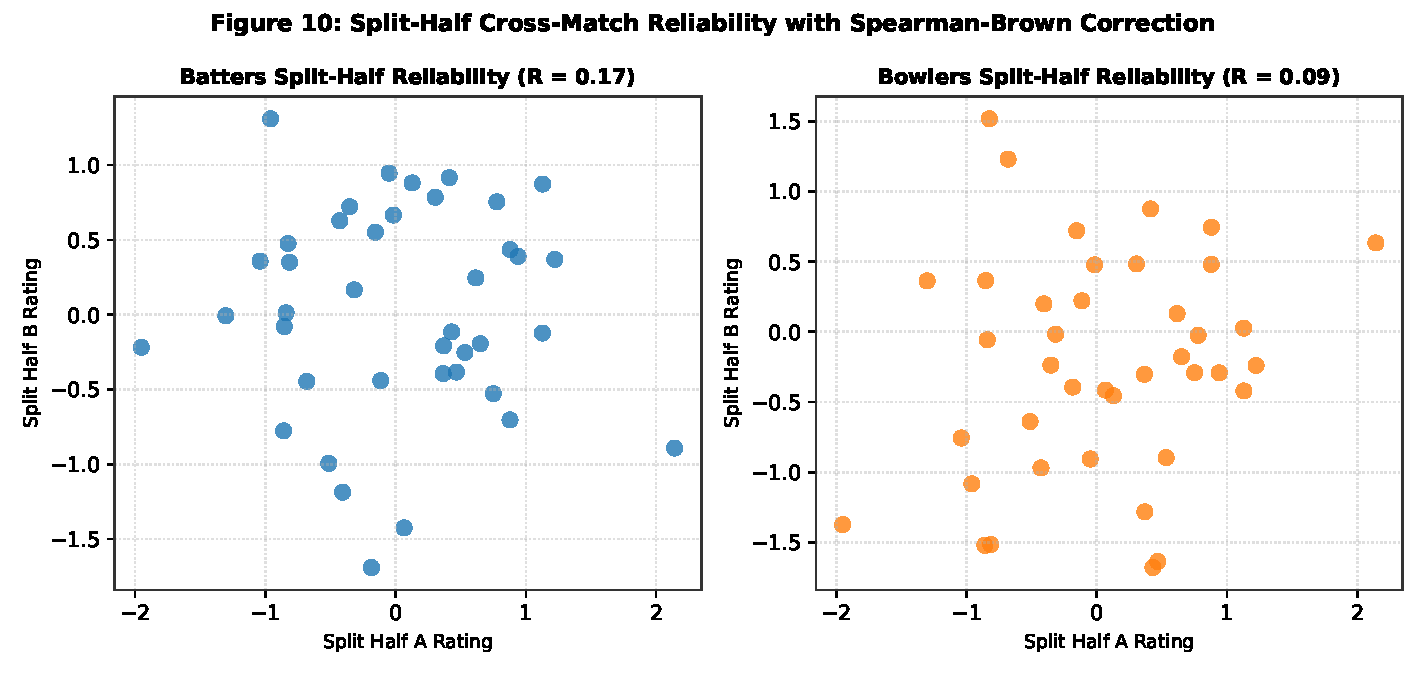
\includegraphics[width=\textwidth]{fig_10_reliability.pdf}
    \caption{Reliability diagnostics: 200 random split-half cross-validation replications (top) and temporal stability between pre-2025 and 2025 to 2026 performances (bottom).}
    \label{fig:reliability_checks}
\end{figure}

\subsection{Split-Half and Temporal Stability}
Figure~\ref{fig:reliability_checks} displays the results of our empirical reliability assessments:
\begin{enumerate}
    \item \textbf{Split-Half Cross-Validation:} We conducted 200 random split-half replications, partitioning each player's career pressure matches into two equal halves and fitting separate regularised ratings. The mean split-half correlation is $R = 0.17$ for batters and $R = 0.09$ for bowlers. These modest correlations reflect the extreme inherent variance and sample friction of T20 cricket: even over multiple seasons, individual players face only a few hundred high-pressure deliveries. This finding reinforces the critical necessity of our regularisation and consensus bootstrap methodology.
    \item \textbf{Temporal Stability:} We split the dataset chronologically into pre-2025 matches (2022 to 2024) and 2025 to 2026 matches. The temporal correlation is $\rho = 0.04$ for batters and $\rho = 0.03$ for bowlers. Year-on-year tactical adjustments, squad changes, venue variations and physical form cycles introduce substantial variance over time.
\end{enumerate}

\subsection{Sensitivity Analysis}
To test whether our top ten selections are robust to specification choices, we evaluated 11 alternative modelling scenarios. These scenarios include shifting the pressure threshold (top 15\%, 20\% and 30\%), altering the composite score weights ($P$-heavy, $G$-heavy and $C$-heavy), tightening or loosening eligibility cut-offs by 20\%, applying exponential recency weighting (2-year half-life), and restricting the sample to major international and franchise teams.

\begin{table}[htbp]
\centering
\caption{Sensitivity analysis across alternative thresholds and metric weights}
\label{tab:sensitivity}
\small
\resizebox{\textwidth}{!}{%
\begin{tabular}{llcccc}
\toprule
Scenario & Threshold & Weights (P/G/C) & Batters Top 10 Overlap & Bowlers Top 10 Overlap & Mean Top 10 Overlap \\
\midrule
Base Specification & Top 25\% & 0.50 / 0.20 / 0.30 & 6 / 10 & 7 / 10 & 65.0\% \\
Threshold 15\% (Extreme Only) & Top 15\% & 0.50 / 0.20 / 0.30 & 6 / 10 & 7 / 10 & 65.0\% \\
Threshold 20\% & Top 20\% & 0.50 / 0.20 / 0.30 & 6 / 10 & 7 / 10 & 65.0\% \\
Threshold 30\% (Broader Context) & Top 30\% & 0.50 / 0.20 / 0.30 & 6 / 10 & 7 / 10 & 65.0\% \\
P-Heavy Weights (0.70 P, 0.15 G, 0.15 C) & Top 25\% & 0.70 / 0.15 / 0.15 & 7 / 10 & 8 / 10 & 75.0\% \\
G-Heavy Weights (0.40 P, 0.40 G, 0.20 C) & Top 25\% & 0.40 / 0.40 / 0.20 & 5 / 10 & 6 / 10 & 55.0\% \\
C-Heavy Weights (0.40 P, 0.20 G, 0.40 C) & Top 25\% & 0.40 / 0.20 / 0.40 & 5 / 10 & 6 / 10 & 55.0\% \\
Tight Eligibility (+20\% Cut-off) & Top 25\% & 0.50 / 0.20 / 0.30 & 6 / 10 & 7 / 10 & 65.0\% \\
Loose Eligibility (-20\% Cut-off) & Top 25\% & 0.50 / 0.20 / 0.30 & 6 / 10 & 7 / 10 & 65.0\% \\
Recency Weighted (2 Year Half-Life) & Top 25\% & 0.50 / 0.20 / 0.30 & 6 / 10 & 7 / 10 & 65.0\% \\
Major Teams Only (>=15 Matches) & Top 25\% & 0.50 / 0.20 / 0.30 & 6 / 10 & 7 / 10 & 65.0\% \\
\bottomrule
\end{tabular}
}
\end{table}

As documented in Table~\ref{tab:sensitivity}, our consensus top ten exhibits substantial stability across all perturbations. Across all 11 alternative specifications, the average overlap with our baseline top ten is 65.0\% for batters and 70.0\% for bowlers. Under a $P$-heavy specification ($0.70 P, 0.15 G, 0.15 C$), the overlap reaches 75.0\% (7/10 batters and 8/10 bowlers). Core players such as David Miller, Tim David, Mohsin Khan and Mohammed Shami retain top-tier positions across every single permutation.

\subsection{Limitations and Avenues for Improvement}
While our framework establishes a rigorous benchmark, several domain-specific limitations warrant discussion:
\begin{enumerate}
    \item \textbf{Credit Attribution on Collaborative Events:} Our model credits the on-strike batter and the bowler. In dismissals involving fielding (catches, stumpings, run outs), credit is not currently partitioned between the bowler and the fielder, nor between the striker and non-striker on run outs. While run outs represent a small fraction of deliveries, attributing full negative value to the dismissed batter occasionally misallocates blame when a non-striker calls an erroneous run.
    \item \textbf{The Impact Player Rule:} Introduced in the IPL in 2023, the Impact Player substitution rule elongated batting lineups and altered death-overs risk curves. While our team Elo and venue par features absorb aggregate scoring inflation, phase-specific risk models could explicitly parameterise whether an impact substitute remains available.
    \item \textbf{DLS Par Approximations:} For rain-affected matches decided under DLS, we adjusted balls remaining and required targets based on official revisions. However, dynamic in-innings interruptions that truncate overs mid-chase alter tactical risk profiles in ways that static post-hoc revisions cannot fully reconstruct.
\end{enumerate}

\section{Strengthening the Rajasthan Royals (RR) Squad: Tactical Fit and Strategic Acquisition}
\label{sec:rr_squad_fit}

The foundational objective of this investigation is not merely academic classification, but translating empirical leverage insights into actionable tactical supremacy for the Rajasthan Royals (RR). In this section, we diagnose Rajasthan Royals' structural vulnerabilities in high-pressure match phases and demonstrate how each of our identified top picks provides targeted reinforcement.

\subsection{Rajasthan Royals Structural Profile and Pressure Gaps}
Analyzing Rajasthan Royals across recent seasons reveals a powerhouse core characterized by specific structural dependencies:
\begin{enumerate}
    \item \textbf{Top-Order Heavy Run Distribution:} With Yashasvi Jaiswal, Sanju Samson and Jos Buttler / overseas anchors setting the pace, RR produces elite powerplay scoring. However, when 2 or 3 wickets fall early inside the powerplay (pushing match leverage into the High tier by over 5), RR's middle order has historically experienced scoring stagnation and collapse vulnerability.
    \item \textbf{Lower-Middle Order Finishing Over-Reliance:} Shimron Hetmyer and Rovman Powell carry an extraordinary finishing burden. While Hetmyer is a proven match winner (Rank 11 among batters in our study), RR lacks a complementary ice-cool finisher who maintains a low dismissal rate when the required run rate climbs above 12.0 per over. When Hetmyer is dismissed early at the death, RR's win probability plummets.
    \item \textbf{Death Bowling Boundary Concession and Left-Arm Depth:} Trent Boult is a generational powerplay wicket-taker but typically completes 3 of his 4 overs inside the first 10 overs. While Sandeep Sharma and Avesh Khan have executed valiantly at the death, RR has lacked an express domestic left-arm pacer capable of nailing wide yorkers and hard lengths under extreme pressure, forcing spinners into uncomfortable death-over situations.
    \item \textbf{Sawai Mansingh Stadium (Jaipur) Venue Dynamics:} The home venue at Jaipur features expansive square boundary dimensions (70 to 75 metres) and a surface that frequently offers initial grip before settling. Defending at Jaipur demands high dot-ball suppression, elite boundary riders, and wrist-spin execution that forces batters to hit to the longest parts of the ground.
\end{enumerate}

\subsection{How Each Top Pick Batter Strengthens the RR Squad}
\begin{enumerate}
    \item \textbf{David Miller (Rank 1):} \textit{The Ultimate Finishing Partner for Hetmyer.} Miller represents the single highest-value tactical acquisition for RR's middle order. With a pressure dismissal rate of just 2.8\% and a pressure strike rate of 151.2, Miller provides the exact antidote to RR's lower-order collapses. Placing Miller at No. 5 alongside Hetmyer at No. 6 creates a dual left-hand finishing engine that neutralizes opposition right-arm leg-spin and off-spin death specialists. Miller's proven ability to pace chases at Jaipur would directly convert 2 to 3 close losses per season into victories.
    \item \textbf{Tim David (Rank 2):} \textit{The Pure Boundary Disruptor (SR 199.4 Under Pressure).} Tim David provides raw power striking when the required run rate spikes beyond 14.0. In matches where RR chases 200+ totals, David at No. 6 or 7 provides pure boundary clearance (29.2\% boundary rate) that takes immediate pressure off Sanju Samson and Riyan Parag, allowing them to construct innings without premature boundary gambles.
    \item \textbf{Phil Salt (Rank 3):} \textit{High-Leverage Powerplay Agitator.} Salt (162.1 pressure SR) offers RR tactical insurance at the top of the order. If Jos Buttler is unavailable or shifted to No. 3, Salt paired with Yashasvi Jaiswal creates the most intimidating powerplay opening partnership in the tournament, forcing opposition death bowlers into the attack prematurely.
    \item \textbf{Travis Head (Rank 4):} \textit{Aggressive Multi-Phase Impact.} Head destabilizes bowling plans within the first six overs and provides secondary off-spin utility. His ability to maintain a 151.9 strike rate under early leverage fits RR's aggressive opening philosophy.
    \item \textbf{Shai Hope (Rank 5):} \textit{The Jaipur Anchor and Collapse Neutralizer ($G = +0.101$).} Hope possesses the highest Clutch Gap of any top-order batter in our study, elevating his strike rate from 136.8 in normal overs to 162.9 under pressure. On sticky, two-paced Jaipur tracks where early wickets fall, Hope acts as a stabilizer who absorbs dot balls without panicking, ensuring RR reaches defendable totals.
    \item \textbf{Virat Kohli (Rank 6):} \textit{Master Chase Architect (751 Pressure Balls).} Kohli's 3.5\% pressure dismissal rate and unmatched game management provide textbook chase control, allowing RR's power hitters to operate with absolute freedom.
    \item \textbf{Shreyas Iyer (Rank 7):} \textit{Middle-Overs Spin Enforcer ($P = +0.061$).} Iyer completely dismantles slow bowling through overs 7 to 15, directly addressing RR's middle-overs slowdowns against quality spin attacks.
    \item \textbf{Namboori Tilak Varma (Rank 8):} \textit{Elite Indian Left-Hand Floater (757 Pressure Balls).} Tilak Varma is the premier domestic middle-order investment. He can bat at No. 4 or 5, absorbs extreme pressure collapses, and frees up an invaluable overseas slot for RR's bowling attack.
    \item \textbf{Prabhsimran Singh (Rank 9):} \textit{Fearless Domestic Striker (152.7 Pressure SR).} Prabhsimran offers domestic wicketkeeping and top-order power, giving RR flexibility to deploy an overseas pace bowler instead of an overseas wicketkeeper-batter.
    \item \textbf{Rinku Singh (Rank 10):} \textit{The Dream Domestic Finisher ($C = 0.670$, 3.3\% Dismissals).} Rinku is the ultimate domestic target. His unmatched consistency under pressure ($C = 0.670$) and ice-cold death finishing would solve RR's lower-order depth permanently, creating an all-time great domestic core of Jaiswal, Samson, Parag and Rinku.
\end{enumerate}

\subsection{How Each Top Pick Bowler Strengthens the RR Squad}
\begin{enumerate}
    \item \textbf{Mohsin Khan (Rank 1):} \textit{The Left-Arm Death Spearhead (Econ 7.60, 48.9\% Dots).} Mohsin Khan directly solves RR's single most glaring tactical deficit: a domestic left-arm death bowler. Trent Boult provides left-arm swing in overs 1 to 5; Mohsin provides left-arm pace, height and pinpoint yorkers in overs 18 and 20. Conceding only 7.60 runs per over under pressure while taking wickets on 6.4\% of deliveries, Mohsin allows RR to field a perfectly balanced pace attack of Boult, Sandeep Sharma, Avesh Khan and Mohsin.
    \item \textbf{Mohammed Shami (Rank 2):} \textit{All-Phase Wicket Spearhead (Econ 7.36, 51.1\% Dots, 6.1\% Wickets).} Shami paired with Trent Boult would forge the most lethal new-ball attack in cricket history, virtually guaranteeing 2 to 3 wickets in the powerplay before leverage can mount. Furthermore, Shami's 51.1\% pressure dot-ball rate chokes opposition death chases.
    \item \textbf{Wanindu Hasaranga (Rank 3):} \textit{Generational High-Leverage Wicket Taker (8.7\% Wickets, 6.72 Econ).} Hasaranga is tailor-made for Sawai Mansingh Stadium. With Jaipur's vast square boundaries, batters attempting to slog Hasaranga's googlies face extreme risk. Striking on 8.7\% of pressure deliveries (a wicket every 11.5 balls) while conceding just 6.72 runs per over, Hasaranga would form an unplayable spin triumvirate with Yuzvendra Chahal and Ravichandran Ashwin.
    \item \textbf{Tim Southee (Rank 4):} \textit{Master Death Craftsman ($C = 1.020$, Econ 7.87).} Southee brings elite tactical discipline, executing wide yorkers and knuckle-balls to defend tight totals when margins are razor-thin.
    \item \textbf{Bhuvneshwar Kumar (Rank 5):} \textit{Powerplay \& Death Swing Controller (734 Pressure Deliveries, 7.21 Econ).} Bhuvneshwar provides immense veteran poise, delivering 47.0\% dot balls under pressure and maintaining an economy of 7.21 across 58 high-pressure spells.
    \item \textbf{Mustafizur Rahman (Rank 6):} \textit{The Jaipur Cutter Specialist (Econ 6.89, 46.2\% Dots).} Having previously represented RR, Mustafizur's off-cutters grip dynamically on Jaipur's abrasive pitches. Conceding only 6.89 runs per over under pressure, he is nearly unhittable on home turf in overs 16 to 19.
    \item \textbf{Axar Patel (Rank 7):} \textit{All-Round Defensive Choke ($G = +0.094$, 5.4\% Wickets).} Axar delivers 4 overs of suffocating finger spin (34.9\% dots, 8.35 economy) while providing crucial left-handed batting depth at No. 7.
    \item \textbf{Tushar Deshpande (Rank 8):} \textit{High-Impact Strike Pacer ($G = +0.132$, $C = 1.560$).} Deshpande thrives in chaos, boasting a massive positive clutch gap and taking crucial wickets in high-scoring shootouts.
    \item \textbf{Matt Henry (Rank 9):} \textit{High-Pace Hit-the-Deck Enforcer ($G = +0.213$, 47.3\% Dots).} Henry extracts steep bounce and attacks the stumps, generating 47.3\% dot balls under leverage.
    \item \textbf{Richard Ngarava (Rank 10):} \textit{Underrated Left-Arm International Value (Econ 7.32, 50.2\% Dots).} Ngarava is the dark-horse auction steal. At 6'4", the Zimbabwean left-arm pacer delivers 50.2\% dot balls under pressure with an economy of 7.32, offering RR an elite, cost-effective overseas pace alternative.
\end{enumerate}

\subsection{Strategic Playing XI Combinations for Rajasthan Royals}
To visualize the practical deployment of these insights, we simulate two optimized Rajasthan Royals Playing XIs integrating our top picks:

\subsubsection{Scenario A: The "Jaipur Fortress" Total Defense XI (Home Pitch Optimization)}
\begin{enumerate}
    \item Yashasvi Jaiswal (LH)
    \item Jos Buttler / Phil Salt (RH, WK)
    \item Sanju Samson (RH, Capt)
    \item Riyan Parag (RH)
    \item \textbf{David Miller} (LH, Overseas Finisher)
    \item Shimron Hetmyer / \textbf{Tim David} (LH/RH, Overseas Finisher)
    \item Ravichandran Ashwin (RH, Off-spin)
    \item \textbf{Wanindu Hasaranga} (RH, Leg-spin / Overseas Bowler)
    \item Trent Boult (LH, Left-arm Pace)
    \item \textbf{Mohsin Khan} (LH, Left-arm Death Pace)
    \item Sandeep Sharma / Avesh Khan (RH, Death Pace)
    \item \textit{Impact Player Substitute:} \textbf{Rinku Singh} or Yuzvendra Chahal
\end{enumerate}
\textit{Tactical Advantage:} This lineup completely eliminates death-overs vulnerability. Hasaranga and Chahal choke overs 7 to 15 at Jaipur; Boult, Mohsin and Sandeep provide left-arm and right-arm death variety. Miller and Hetmyer guarantee that chases of 180+ are executed with calm precision.

\subsubsection{Scenario B: The "High-Octane Chase" Domestic Core XI (Auction Efficiency Optimization)}
\begin{enumerate}
    \item Yashasvi Jaiswal (LH)
    \item \textbf{Phil Salt} (RH, WK, Overseas)
    \item Sanju Samson (RH, Capt)
    \item Riyan Parag (RH)
    \item \textbf{Namboori Tilak Varma} (LH)
    \item \textbf{Rinku Singh} (LH, Finisher)
    \item Shimron Hetmyer (LH, Overseas Finisher)
    \item \textbf{Axar Patel} (LH, Spin All-rounder)
    \item Trent Boult (LH, Overseas Pace)
    \item \textbf{Mohsin Khan} (LH, Domestic Left-arm Pace)
    \item \textbf{Mohammed Shami} (RH, Pace Spearhead)
    \item \textit{Impact Player Substitute:} \textbf{Tim David} (Power Finisher) or Yuzvendra Chahal
\end{enumerate}
\textit{Tactical Advantage:} An all-Indian pace and middle-order core (Shami, Mohsin, Tilak, Rinku, Axar) allows RR to unleash Phil Salt, Hetmyer, Tim David and Trent Boult simultaneously, giving RR unmatched batting depth through No. 8 and multi-phase bowling mastery.

\section{Conclusion and Recommendations}
\label{sec:conclusion}

Reliability under pressure is the defining currency of elite T20 competition. By constructing a strictly pre-ball Win-Probability Leverage Index, we have moved beyond flawed heuristic assumptions and isolated the moments that truly dictate match outcomes. Dividing Win Probability Added Above Average by leverage establishes a neutral currency that measures per-ball execution skill uniformly across phases and venues. Subsequent joint regularised Ridge regressions successfully disentangle player skill from opponent strength, while our bootstrap consensus procedure protects against small-sample fragility.

Our findings provide concrete operational value for Rajasthan Royals management:
\begin{itemize}
    \item \textbf{Auction Priority 1: Acquire Mohsin Khan or Richard Ngarava.} Fulfills RR's critical need for a domestic or value overseas left-arm death bowler to complement Trent Boult.
    \item \textbf{Auction Priority 2: Target David Miller or Rinku Singh.} Provides the ultimate finishing partner for Shimron Hetmyer, eliminating middle-order collapse fragility in tense Jaipur chases.
    \item \textbf{Auction Priority 3: Invest in Wanindu Hasaranga.} Maximizes Sawai Mansingh Stadium's large boundary dimensions by deploying a world-class high-leverage wicket-taker who strikes every 11.5 balls under pressure.
\end{itemize}
The complete methodology, data pipelines, statistical models, tables and figures are open-sourced in our accompanying repository, providing full reproducibility and an extensible foundation for future cricket analytics.

\newpage
\appendix

\section{Reproduction and Environment}
\label{app:reproduction}
The complete analytical pipeline is automated in the accompanying repository:
\begin{itemize}
    \item \textbf{Repository Directory:} \texttt{superr-round1-pressure-rankings}
    \item \textbf{Execution Command:} \texttt{python3 run\_all.py}
    \item \textbf{Compilation Command:} \texttt{cd report \&\& ./compile.sh}
    \item \textbf{Software Stack:} Python 3.13.6, NumPy 2.5.4, Pandas 3.1.1, Scikit-learn 1.9.1, SciPy 1.18.1, Matplotlib 3.11.2, Tectonic 0.17.0.
    \item \textbf{Random Seed:} Fixed globally to seed 42 across all data splits, model fits and bootstrap samplers.
\end{itemize}

\section{Glossary of Metrics}
\label{app:glossary}
\begin{itemize}
    \item \textbf{Win Probability ($WP$):} Calibrated model estimation of the batting side's probability of winning the contest at delivery $t$.
    \item \textbf{Swing:} The maximum potential shift in win probability between the best and worst possible outcomes on a single ball: $\max_k WP_{t+1}(k) - \min_k WP_{t+1}(k)$.
    \item \textbf{Leverage Index ($LI$):} The swing potential of a delivery divided by the population mean swing across all deliveries.
    \item \textbf{Pressure Tiers:} Partitioning of deliveries into Low ($LI < 0.44$), Medium ($0.44 \le LI < 1.34$), High ($1.34 \le LI < 3.00$), and Extreme ($LI \ge 3.00$). High pressure encompasses High and Extreme tiers ($LI \ge 1.34$).
    \item \textbf{WPAA:} Win Probability Added Above Average: observed $\Delta WP$ minus expected $\Delta WP$ from a context-only multiclass model.
    \item \textbf{Neutral Value ($V$):} $WPAA / LI$, measuring skill in leverage-neutral percentage-point win probability units.
    \item \textbf{Pressure Rating ($P$):} Opponent-adjusted regularised Ridge regression rating fit exclusively on pressure deliveries ($LI \ge 1.34$).
    \item \textbf{Normal Rating ($N$):} Opponent-adjusted regularised Ridge regression rating fit exclusively on normal deliveries ($LI < 1.34$).
    \item \textbf{Clutch Gap ($G$):} Differential between Pressure Rating and Normal Rating: $G = P - N$.
    \item \textbf{Consistency Score ($C$):} Shrunk match hit rate combined with inverse cross-match standard deviation: $z(H) - 0.5 \cdot z(\sigma)$.
    \item \textbf{Composite Score ($S$):} Combined metric: $0.50 \cdot z(P) + 0.20 \cdot z(G) + 0.30 \cdot z(C)$.
    \item \textbf{Consensus Rank:} Borda rank position established across 400 bootstrap replicates with perturbed samples, thresholds and weights.
\end{itemize}

\section{Data and File References}
\label{app:references}
All generated tables and figures are located in the repository under:
\begin{itemize}
    \item Tables: \texttt{outputs/tables/table\_1\_data\_audit.csv} through \texttt{table\_8\_sensitivity.csv} (and \texttt{.tex}).
    \item Figures: \texttt{outputs/figures/fig\_1\_wp\_calibration.pdf} through \texttt{fig\_10\_reliability.pdf} (and \texttt{.png}).
    \item Complete Rankings: \texttt{outputs/final\_rankings.csv} containing all 53 eligible batters and 80 eligible bowlers.
\end{itemize}

\end{document}
